% Template for an EarthArXiv preprint of the manuscript.
% Includes the standard disclaimers and formatting that is required.
%
% This is the document structure. The actual content is written in:
% * abstract.tex: The abstract.
% * abstract-plain.tex: A plain language version of the abstract.
% * content.tex: The actual manuscript text (minus the abstract).
%
%%%%%%%%%%%%%%%%%%%%%%%%%%%%%%%%%%%%%%%%%%%%%%%%%%%%%%%%%%%%%%%%%%%%%%%%%%%%%%%
% Set a class and general configuration
\documentclass[onecolumn,10pt]{article}

%%%%%%%%%%%%%%%%%%%%%%%%%%%%%%%%%%%%%%%%%%%%%%%%%%%%%%%%%%%%%%%%%%%%%%%%%%%%%%%
% Set variables with the title, authors, etc.
\newcommand{\Title}{Euler inversion: Locating sources of potential-field data through inversion of Euler's homogeneity equation}
\newcommand{\TitleShort}{Euler inversion}

\newcommand{\Year}{2024}
\newcommand{\SubmittedOn}{2023/02/28}
\newcommand{\PublishedOn}{2023/02/28}

\newcommand{\AuthorShort}{Uieda et al.}
\newcommand{\Authors}{%
  Leonardo Uieda\textsuperscript{1},
  Gelson Ferreira Souza-Junior\textsuperscript{1},
  India Uppal\textsuperscript{2},
  Vanderlei Coelho Oliveira Jr.\textsuperscript{3},
  Valéria Cristina Ferreira Barbosa\textsuperscript{3}
}
\newcommand{\Email}{uieda@usp.br}
\newcommand{\Corresponding}{%
  Corresponding author: Leonardo Uieda <\href{mailto:\Email}{\Email}>
}
\newcommand{\Affiliations}{%
  \textsuperscript{1} Universidade de São Paulo, Brazil;
  \textsuperscript{2} University of Liverpool, UK;
  \textsuperscript{3} Observatório Nacional, Brazil;
}

\newcommand{\Journal}{Geophysical Journal International}
\newcommand{\JournalDOI}{YYYYY/YYYYYYY}
\newcommand{\PreprintDOI}{XXXXX/XXXXXXX}
\newcommand{\ArchiveDOI}{DOI_FOR_THE_REPO_ARCHIVE}
\newcommand{\GitHubRepository}{compgeolab/euler-inversion}

\newcommand{\Keywords}{%
  keyword1; keyword2; keyword3;
}

%%%%%%%%%%%%%%%%%%%%%%%%%%%%%%%%%%%%%%%%%%%%%%%%%%%%%%%%%%%%%%%%%%%%%%%%%%%%%%%
% Import the required packages
\usepackage[utf8]{inputenc}
\usepackage[TU]{fontenc}
\usepackage[english]{babel}
\usepackage{amsmath}
\usepackage{amssymb}
\usepackage{graphicx}
\usepackage{hyperref}
\usepackage{fancyhdr}
\usepackage{orcidlink}
\usepackage{geometry}
\usepackage{booktabs}
\usepackage{microtype}
\usepackage{siunitx}
\usepackage[longend,linesnumbered,ruled]{algorithm2e}
% To customize the title page
\usepackage{titling}
% For adding multiple authors
\usepackage{authblk}
% improved urls with proper hyphenation
\usepackage{xurl}
% Tweak the look of captions
\usepackage{caption}
% To control the style of section titles
\usepackage{titlesec}
% Import natbib and doi packages
\usepackage[round,authoryear,sort]{natbib}
% show dois as links on references
\usepackage{doi}
% Remove extra space between references
\usepackage{natbibspacing}
% Use a different font
\usepackage[scaled=1.1]{notomath}
% Icons and fonts (requires using xelatex or luatex)
\usepackage{fontawesome5}
\usepackage{academicons}
% Control the font size
\usepackage{anyfontsize}
\usepackage{setspace}
% To get the number of pages in the document
\usepackage{lastpage}
\usepackage{lipsum}
\usepackage{ragged2e}
\usepackage{mdframed}
% To define custom environments
\usepackage{environ}
% To control hyphenation for individual blocks of text
\usepackage{hyphenat}


%%%%%%%%%%%%%%%%%%%%%%%%%%%%%%%%%%%%%%%%%%%%%%%%%%%%%%%%%%%%%%%%%%%%%%%%%%%%%%%
% Math shortcuts

% To be able to use matrices with more than 10 columns in amsmath
\setcounter{MaxMatrixCols}{20}

% Lagrangian
\DeclareMathOperator{\Lagr}{\mathcal{L}}
% Merit function
\DeclareMathOperator{\Merit}{\mathcal{M}}


%%%%%%%%%%%%%%%%%%%%%%%%%%%%%%%%%%%%%%%%%%%%%%%%%%%%%%%%%%%%%%%%%%%%%%%%%%%%%%%
% Configuration of the document

\geometry{%
  left=25mm,
  right=25mm,
  top=18mm,
  bottom=15mm,
  headsep=0mm,
  headheight=0mm,
  footskip=7mm,
  includehead=true,
  includefoot=true
}

% Control line and table row spacing
\onehalfspacing
\renewcommand{\arraystretch}{1.5}

% Set the spacing between bibliography entries (requires natbib)
\setlength{\bibsep}{0pt}

% Custom colors
\definecolor{darkgray}{gray}{0.4}
\definecolor{mediumgray}{gray}{0.5}
\definecolor{lightgray}{gray}{0.9}
\definecolor{mediumblue}{HTML}{2060c2}
\definecolor{lightblue}{HTML}{f7faff}

% Configure captions
\captionsetup[table]{position=below,skip=0pt}
\captionsetup{labelfont=bf,font={small,color=darkgray},skip=10pt}

% Make urls use the same font as every other text
\urlstyle{same}

% Configure hyperref and add PDF metadata
\hypersetup{
    colorlinks,
    allcolors=mediumblue,
    pdftitle={\Title},
    pdfauthor={\AuthorShort},
    breaklinks=true,
}

% Configure header and footer
% Inspired by LaPreprint: https://github.com/roaldarbol/LaPreprint
\newcommand{\Separator}{\hspace{3pt}|\hspace{3pt}}
\newcommand{\FooterFont}{\footnotesize\color{mediumgray}}
\pagestyle{fancy}
\fancyhf{}
\lfoot{%
  \FooterFont{}
  \AuthorShort{} (\Year)
  \Separator{}
  \TitleShort
}
\rfoot{%
  \FooterFont{}
  EarthArXiv
  \Separator{}
  \thepage\space of\space \pageref*{LastPage}
}
\renewcommand{\headrulewidth}{0pt}
\renewcommand{\footrulewidth}{1pt}
\preto{\footrule}{\color{lightgray}}
\fancypagestyle{plain}{%
  \fancyhf{}
  \lfoot{%
    \FooterFont{}
    \faCreativeCommons\faCreativeCommonsBy
    \Separator{}
    \textcopyright{} \Year{} The Authors
  }
  \rfoot{%
    \FooterFont{}
    doi:\href{https://doi.org/\PreprintDOI}{\PreprintDOI}
    \Separator{}
    EarthArXiv
    \Separator{}
    \thepage\space of\space \pageref*{LastPage}
  }
}

% Define fancy text boxes
\NewEnviron{summarybox}{%
  \mdfdefinestyle{summarybox_}{%
    leftline=true,
    rightline=false,
    topline=false,
    bottomline=false,
    linewidth=2pt,
    linecolor=mediumblue,
    backgroundcolor=lightblue,
    innertopmargin=12pt,
    innerbottommargin=12pt,
    innerleftmargin=12pt,
    innerrightmargin=12pt,
    skipbelow=5pt,
    skipabove=5pt,
  }
  \newmdenv[style=summarybox_]{summarybox_}
  \begin{summarybox_}
    \footnotesize
    \BODY
  \end{summarybox_}
}

%%%%%%%%%%%%%%%%%%%%%%%%%%%%%%%%%%%%%%%%%%%%%%%%%%%%%%%%%%%%%%%%%%%%%%%%%%%%%%%
\begin{document}

\thispagestyle{plain}
\begin{FlushLeft}
  \begin{spacing}{2}
    {\LARGE\bfseries \Title}
  \end{spacing}
  {\color{lightgray}\hrule height 1.5pt}
  \vspace{0.3cm}
  \Authors
  \\[0.2cm]
  {\footnotesize \Affiliations}
  \newline
  {\footnotesize \Corresponding}
  \\[0.2cm]
  {\footnotesize
    Received in original form on \SubmittedOn.
    %Published in final form on \PublishedOn.
  }
\end{FlushLeft}

\begin{summarybox}
  \noindent
  \textbf{Disclaimer:}
  This is a non-peer reviewed preprint of an article submitted for publication
  in \textit{\Journal{}}. It is available from EarthArXiv at
  \url{https://doi.org/\PreprintDOI}.
  %%%%%%%%%%%%%%%%%%%%%%%%%%%%%%%%%%%%%%%%%%%%%%%%%%%%%%%%%%%%%%%%%%%%%%%%%%%%%
  % Comment the above and uncomment below after publication in a journal
  %%%%%%%%%%%%%%%%%%%%%%%%%%%%%%%%%%%%%%%%%%%%%%%%%%%%%%%%%%%%%%%%%%%%%%%%%%%%%
  %This is a peer-reviewed author-produced postprint of the article
  %``\AuthorShort{} (\Year). \Title. \textit{\Journal}.
  %doi:\href{https://doi.org/\JournalDOI}{\JournalDOI}''.
  %The postprint is available from EarthArXiv at
  %\url{https://doi.org/\PreprintDOI}.
  %%%%%%%%%%%%%%%%%%%%%%%%%%%%%%%%%%%%%%%%%%%%%%%%%%%%%%%%%%%%%%%%%%%%%%%%%%%%%
  \\[0.25cm]
  \noindent
  \textbf{Open research:}
  The source code used to generate all of the results presented in this
  research can be freely accessed and reused under the terms of an open license.
  You can find it at \url{https://doi.org/\ArchiveDOI} and
  \url{https://github.com/\GitHubRepository}.
  \\[0.25cm]
  \noindent
  \textbf{Keywords:} \Keywords{}
  \\[0.25cm]
  \noindent
  \textbf{\textcopyright{} \Year{} The Authors.}
  Available under the \href{https://creativecommons.org/licenses/by/4.0/}{Creative Commons Attribution 4.0 International License}
  \faCreativeCommons\faCreativeCommonsBy{}.
\end{summarybox}

\section*{\normalsize Plain language summary}
\begingroup
  \setstretch{1.1} \small Earth scientists are able to determine the depth of certain rocks in below ground by measuring the small disturbances that they cause to Earth's gravity and magnetic fields.
A popular method for doing this is \textit{Euler deconvolution}, which is widely available in geoscience software and is fast to run on an average computer. 
Unfortunately, Euler deconvolution has some shortcomings: 1) the approximate shape of the rocks must be known, for example a sphere or a wide flat slab, which is represented by something called the \textit{structural index} 2) the depth of the rocks is not well estimated when there is noise in our data, which is a common occurrence.
We propose a new method that uses more adequate (and complex) mathematics to fix some of the shortcomings of Euler deconvolution.
We call our new method \textit{Euler inversion}.
It is less sensitive to noise in the data and is also able to determine the approximate shape of the source (the structural index).
Our new method is able to replace Euler deconvolution on an Earth scientists toolbox because it is also fast to execute on an average computer. \par
\endgroup

\section*{\normalsize Abstract}
\begingroup
  \setstretch{1.1} \small Locating the sources of observed disturbances in potential-field data is a challenging problem due to the non-unique nature of the inverse problem.
The Euler deconvolution method was created to solve this issue, particularly for idealized sources (such as spheres and planar vertical dykes).
Euler deconvolution has become widely used in potential-field methods due, in large part, to its low computational cost and ease of implementation into software.
However, it is widely known that Euler deconvolution suffers from some shortcomings: 1) non-uniqueness of the solution with respect to the depth of the source and the structural index (a parameter that represents the idealised shape of the source); 2) sensitivity to short-wavelength noise in the data derivatives which are used as inputs for the method.
Here, we present a new method called \textit{Euler inversion} which is a reformulation of the inverse problem of Euler's homogeneity equation as an implicit mathematical model rather than a parametric one.
Euler inversion is a constrained, non-linear inverse problem capable of estimating both the model parameters (location of the source and constant base level) and the predicted data (potential field and its derivatives).
We show that Euler inversion is less sensitive than Euler deconvolution to short-wavelength noise and to the presence of interfering sources in the data window.
By also estimating the predicted data, Euler inversion is also able to estimate the best integer structural index
to be used for inversion.
Our results show that the estimated structural index minimizes the data misfit and coincides with those of the simulated sources.
Furthermore, most matrices involved in the method are either sparse or diagonal, making Euler inversion computationally efficient.
Tests on synthetic data and a real aeromagnetic dataset from Rio de Janeiro, Brazil, demonstrate the effectiveness of Euler inversion to delineate sources with variable geometries and correctly estimate their depths.
 \par
\endgroup

\section{Introduction}

Estimating the depths of the sources of measured anomalies is a common challenge in potential-field geophysics.
One of the most widely used techniques for providing depth estimates is Euler deconvolution \citep{Thompson1982,Reid1990}.
Its widespread adoption is due, in large part, to its low algorithmic complexity and fast computation times, both of which are orders of magnitude smaller than solutions from 3D inverse problems.
As a result, Euler deconvolution is widely available in both commercial and open-source software \citep{Uieda2013,Uieda2014}.
Unfortunately, this popularity has also led to abuses of the method, as reported in \citet{Reid2014} and \citet{Reid2014b}.

Euler deconvolution is a method that assumes potential-field data are generated by idealized sources, such as dikes, dipoles, or pipes.
The geometry of these sources is characterized by the structural index, a parameter that must be an integer to retain physical significance
\citep{Stavrev2007,Reid2014}.
The technique involves performing a least-squares inversion of Euler's homogeneity equation multiple times, in a moving window scheme.
Each inversion estimates the base level, a constant shift in the data, and also the coordinates of a single idealized source
potentially present within the study area.

It is well known that Euler deconvolution suffers from some limitations, of which we highlight:

\begin{enumerate}

\item \textbf{Separation of reliable and spurious solutions:}
The moving window scheme adopted in Euler deconvolution generates many estimated positions which are considered spurious and must be removed.
Most of the spurious solutions happen when the moving window either lacks significant potential-field anomalies or only contains
a truncated anomaly.
\citet{FitzGerald2004} and \citet{Melo2020} provide overviews of the many existing methods that have been developed to remove spurious solutions.

\item \textbf{Sensitivity to high-frequency noise:} Random noise in the data is usually of high-frequency, which gets amplified in the derivative calculations. Since the field derivatives are used in the Jacobian matrix of the least-squares inversions, errors in the derivatives will have a large impact on the solution.
\citet{Pasteka2009}, \citet{Saleh2012}, and \citet{Florio2014} recommend using regularised derivatives or other smoothing techniques to reduce the noise amplification and obtain more reliable solutions.
This is also why Euler deconvolution variants that rely on higher-order derivatives, like tilt-Euler deconvolution \citep{Salem2007,Huang2019} and AN-EUL \citep{Salem2003}, present a larger dispersion of estimated positions and are more sensitive to noise in general.
Methods like finite-difference Euler deconvolution \citep{Gerovska2005} and ratio-Euler deconvolution \citep{Huang2022} were specifically developed to avoid the use of higher-order derivatives because of this noise-sensitivity issue.

\item \textbf{Correlation of the estimated depth and the structural index:}
\citet{Silva2001} demonstrated that the estimated depth from Euler deconvolution is directly correlated with the structural index used.
The higher the structural index, the larger the estimated depth.
This makes it very important to know the best integer structural index for the type of source being interpreted.
Some Euler deconvolution variants have been developed that are able to estimate the structural index \citep[e.g.,][]{Melo2013,Melo2018,Salem2003,Salem2007,Gerovska2005,Silva2003,Florio2013,Florio2014}.
However, most of them estimate real-valued structural indices instead of integers, are sensitive to noise, and tend to underestimate the structural index under realistic noise and signal overlap scenarios.

\end{enumerate}

We aim to tackle the issues of sensitivity to noise and structural index estimation by reformulating the inverse problem of solving Euler's homogeneity equation.
The issue of noise sensitivity can be traced back to the presence of data derivatives in the Jacobian matrix, which generally contain larger amounts of noise than the original potential field.
We propose formulating the inverse problem as a non-linear optimisation with Euler's equation as a constraint.
This is similar to ``total least-squares'' in statistics \citep{VanHuffel1991} and ``combined adjustment'' in geodesy \citep{Vanicek1986}.
Another advantage of this new formulation is the ability to calculate predicted data for the potential-field and its three derivatives, which is impossible in Euler deconvolution and all of its variants.
We call our new method ``Euler inversion''.

%%%%%%%%%%%%%%%%%%%%%%%%%%%%%%%%%%%%%%%%%%%%%%%%%%%%%%%%%%%%%%%%%%%%%%%%%%%%%%%
\section{Methodology}

Starting with \citet{Thompson1982} and \citet{Reid1990}, Euler's equation has
been used to estimate the source positions of gravity and magnetic data.
In this section, we will review the solution of Euler's equation for
the source location $(x_o, y_o, z_o)$ by Euler deconvolution \citep{Reid1990} and then present a
new method, called \textit{Euler inversion}, for solving Euler's equation using
total least-squares.

We start with Euler's homogeneity equation

\begin{equation}
  (x - x_o)\partial_x f + (y - y_o)\partial_y f + (z - z_o)\partial_z f
  + \eta(f - b) = 0
  \ ,
  \label{eq:euler}
\end{equation}

\noindent
in which $f$ is a homogeneous function (in this case, a potential-field),
$\partial_\alpha$ is the derivative operator in the $\alpha$ direction,
$(x, y, z)$ are the coordinates of the observation point,
$(x_o, y_o, z_o)$ are the coordinates of the field source,
$b$ is the base level representing a constant shift in the field,
and $\eta$ is the structural index, which is related to the nature of the
source and how its potential-field values decay with distance
\citep{Ruddock1966,Reid2014}.
The coordinate system is defined with $x$ pointing eastward, $y$ pointing northward, and $z$ pointing upward.
Equation~\ref{eq:euler} relates the coordinates of the source with the
potential field and its gradient observed at the point $(x, y, z)$.

Given $N$ observations points in which we have measured $f$ and its gradient
(for a total $4N$ data), we can define the system of $N$ equations and $4$
unknowns

\begin{equation}
  \begin{aligned}
    (x_1-x_o)\partial_x f_1 + (y_1-y_o)\partial_y f_1 + (z_1-z_o)\partial_z f_1 + \eta(f_1-b) &= 0
    \\
    (x_2-x_o)\partial_x f_2 + (y_2-y_o)\partial_y f_2 + (z_2-z_o)\partial_z f_2 + \eta(f_2-b) &= 0
    \\
    \vdots
    \\
    (x_N-x_o)\partial_x f_N + (y_N-y_o)\partial_y f_N + (z_N-z_o)\partial_z f_N + \eta(f_N-b) &= 0
  \end{aligned}
  \ .
  \label{eq:euler-system}
\end{equation}

\noindent
Both Euler deconvolution and Euler inversion aim to solve the equation system
above to estimate the parameter vector

\begin{equation}
  \mathbf{p} = \begin{bmatrix}x_o & y_o & z_o & b \end{bmatrix}^T.
  \label{eq:p}
\end{equation}


\subsection{Euler deconvolution}

Euler deconvolution starts by rearranging Equation~\ref{eq:euler-system} to
place the parameters on the left-hand side and all other terms on the
right-hand side. This is an attempt to form a \textit{parametric model} which
results in the equation system

\begin{equation}
  \begin{aligned}
  -x_o\partial_x f_1 - y_o\partial_y f_1 - z_o\partial_z f_1 - \eta b &= -x_1\partial_x f_1 - y_1\partial_y f_1 - z_1\partial_z f_1 - \eta f_1
  \\
  -x_o\partial_x f_2 - y_o\partial_y f_2 - z_o\partial_z f_2 - \eta b &= -x_2\partial_x f_2 - y_2\partial_y f_2 - z_2\partial_z f_2 - \eta f_2
  \\
  \vdots
  \\
  -x_o\partial_x f_N - y_o\partial_y f_N - z_o\partial_z f_N - \eta b &= -x_N\partial_x f_N - y_N\partial_y f_N - z_N\partial_z f_N - \eta f_N
  \end{aligned}
  \ ,
\end{equation}

\noindent
which can be written in matrix form as

\begin{equation}
  \underbrace{
    \begin{bmatrix}
      -\partial_x f_1 & -\partial_y f_1 & -\partial_z f_1 & -\eta \\
      -\partial_x f_2 & -\partial_y f_2 & -\partial_z f_2 & -\eta \\
      \vdots & \vdots & \vdots & \vdots \\
      -\partial_x f_N & -\partial_y f_N & -\partial_z f_N & -\eta
    \end{bmatrix}
  }_{\mathbf{A}}
  \underbrace{
    \begin{bmatrix}
      x_o \\ y_o \\ z_o \\ b
    \end{bmatrix}
  }_{\mathbf{p}}
  =
  \underbrace{
    \begin{bmatrix}
      -x_1\partial_x f_1 - y_1\partial_y f_1 - z_1\partial_z f_1 - \eta f_1 \\
      -x_2\partial_x f_2 - y_2\partial_y f_2 - z_2\partial_z f_2 - \eta f_2 \\
      \vdots \\
      -x_N\partial_x f_N - y_N\partial_y f_N - z_N\partial_z f_N - \eta f_N \\
    \end{bmatrix}
  }_{\mathbf{c}}
  \ ,
  \label{eq:deconv-system}
\end{equation}

\noindent
in which $\mathbf{A}$ is the Jacobian matrix of Euler's equation
(Equation~\ref{eq:euler}) concerning the parameters
(Equations~\ref{eq:p})
and $\mathbf{c}$ is a \textit{pseudo-data vector}.

The solution proposed by \citet{Thompson1982} and \citet{Reid1990} is a
least-squares estimate of $\mathbf{p}$

\begin{equation}
  \hat{\mathbf{p}} = \left(\mathbf{A}^T\mathbf{A}\right)^{-1}
  \mathbf{A}^T\mathbf{c}
  \ .
  \label{eq:deconv-p}
\end{equation}

\noindent
The covariance matrix of the solution $\mathbf{C}_p$ is obtained through
standard error propagation assuming that the only variable with uncertainty
is the pseudo-data vector $\mathbf{c}$

\begin{equation}
  \mathbf{C}_p = \hat{\sigma}_0^2 \left(\mathbf{A}^T\mathbf{A}\right)^{-1}
  \ ,
  \label{eq:deconv-cov}
\end{equation}

\noindent
in which
${\hat{\sigma}_0^2} = \|\mathbf{c} - \mathbf{A}\mathbf{p}\|^2 / (N - 4)$
is the reduced chi-squared statistic and an estimate of the variance factor of
$\mathbf{c}$.

The solution in Equation~\ref{eq:deconv-p} above is valid only if the
contents of the Jacobian matrix $\mathbf{A}$ are assumed to be error-free.
As can be seen from Equation~\ref{eq:deconv-system}, the Jacobian contains the
derivatives of $f$, which are often computed numerically by finite-differences
or Fourier transforms and are known to amplify the high-frequency random noise
in the data.
This presents a problem, particularly for the estimation of $z_o$, which has
been widely explored in the literature
\citep{Silva2001,Melo2020,Pasteka2009,Florio2014}.


\subsection{Euler inversion: Formulation}

Euler inversion starts by assigning the potential-field $f$ to a $N \times 1$
vector

\begin{equation}
  \mathbf{f} =
  \begin{bmatrix}
    f_1 & f_2 & \cdots & f_N
  \end{bmatrix}^T.
\end{equation}

\noindent
We can then define a $4N \times 1$ \textit{data vector} which contains all of
the values of $f$ and its gradient

\begin{equation}
  \mathbf{d} =
  \begin{bmatrix}
    \mathbf{f}^T
    & \mathbf{\nabla}_x\mathbf{f}^T
    & \mathbf{\nabla}_y\mathbf{f}^T
    & \mathbf{\nabla}_z\mathbf{f}^T
  \end{bmatrix}^T.
  \label{eq:d}
\end{equation}

\noindent
in which $\mathbf{\nabla}_\alpha$ is the gradient operator in the $\alpha$
dimension.

Next, we formulate the $N \times 4$ equation system
from Euler's equation
(Equation~\ref{eq:euler-system})
as a non-linear function of both parameters and data

\begin{equation}
  \mathbf{e}(\mathbf{p}, \mathbf{d}) = \mathbf{0}
  \ ,
  \label{eq:e}
\end{equation}

\noindent
which is known in geodesy as an \textit{implicit mathematical model}
\citep{Vanicek1986}.

We then wish to solve the following constrained optimisation problem with
non-linear equality constraints to estimate both the parameters and the
predicted data simultaneously

\begin{equation}
  \begin{aligned}
    \min_{\mathbf{p}, \mathbf{d}} \quad &
      \phi(\mathbf{d}) =
      \left[\mathbf{d}^o - \mathbf{d}\right]^T \mathbf{W}
      \left[\mathbf{d}^o - \mathbf{d}\right]
    \\
    \textrm{subject to} \quad &
      \mathbf{e}(\mathbf{p}, \mathbf{d}) = \mathbf{0}
    \ ,
  \end{aligned}
  \label{eq:constrained}
\end{equation}

\noindent
in which $\mathbf{d}^o$ is the \textit{observed data vector} which contains all
of the $4N$ observations of $f$ and its gradient,
$\mathbf{d}$ is the \textit{predicted data vector} from Equation~\ref{eq:d},
and $\mathbf{W}$ is a $4N \times 4N$ diagonal weight matrix.
The first $N$ terms of the diagonal of $\mathbf{W}$ are the weights for the
potential field observations and the following $3N$ terms are the weights of
x-, y-, and z-derivatives of the potential field, in order.

The constrained problem in Equation~\ref{eq:constrained} can be transformed
into an unconstrained problem by using the Lagrangian

\begin{equation}
  \Lagr(\mathbf{p}, \mathbf{d}, \boldsymbol{\lambda}) =
    \left[\mathbf{d}^o - \mathbf{d}\right]^T \mathbf{W}
    \left[\mathbf{d}^o - \mathbf{d}\right]
    +
    2 \boldsymbol{\lambda}^T \mathbf{e}
  \ ,
  \label{eq:lagrangian}
\end{equation}

\noindent
in which $\boldsymbol{\lambda}$ is an $N \times 1$ vector of Lagrange
multipliers.
The non-linear Lagrangian is minimised through Newton's method
\citep{Aster2018}.
We start with initial estimates $\mathbf{p}_0$ and $\mathbf{d}_0$ and then
iteratively apply corrections $\mathbf{\Delta p}_k$ and $\mathbf{\Delta d}_k$
until convergence is achieved.
To calculate the corrections, we introduce a new variable $\mathbf{u} =
[\mathbf{d}^T\  \boldsymbol{\lambda}^T \ \mathbf{p}^T]^T$, expand the
Lagrangian $\Lagr(\mathbf{u})$ (Equation~\ref{eq:lagrangian}) in a Taylor
series around point $\mathbf{u}_k$, and disregard terms of order higher than
two

\begin{equation}
  \Lagr(\mathbf{u}) \approx
  \Gamma(\mathbf{u}) =
  \Lagr(\mathbf{u}_k)
    + \mathbf{\Delta u}_k^T \mathbf{\nabla}\Lagr(\mathbf{u}_k)
    + \dfrac{1}{2}\mathbf{\Delta u}_k^T\mathbf{H}_k\mathbf{\Delta u}_k
  \ ,
  \label{eq:taylor}
\end{equation}

\noindent
in which $\mathbf{\nabla}$ is the gradient operator and $\mathbf{H}_k$ is the
Hessian matrix of $\Lagr$ evaluated at $\mathbf{u}_k$.
Equation~\ref{eq:taylor} is a quadratic function of $\mathbf{\Delta u}_k$ and
we can obtain its minimum by taking its gradient and equating it to the null
vector

\begin{equation}
  \begin{gathered}
    \mathbf{\nabla}\Gamma(\mathbf{\Delta u}_k) =
      \mathbf{\nabla}\Lagr(\mathbf{u_k})
      + \mathbf{H}_k\mathbf{\Delta u}_k
      = \mathbf{0}
    \ ,
    \\
    \mathbf{H}_k\mathbf{\Delta u}_k = -\mathbf{\nabla}\Lagr(\mathbf{u_k})
    \ .
  \end{gathered}
\end{equation}

\noindent
The equation above is the \textit{system of normal equations}, which can also
be written in terms of $\mathbf{p}$, $\boldsymbol{\lambda}$, and $\mathbf{d}$

\begin{equation}
  \underbrace{
    \begin{bmatrix}
      \mathbf{H}^{dd}_k & \mathbf{H}^{d\lambda}_k & \mathbf{H}^{dp}_k \\
      \mathbf{H}^{\lambda d}_k & \mathbf{H}^{\lambda\lambda}_k & \mathbf{H}^{\lambda p}_k \\
      \mathbf{H}^{pd}_k & \mathbf{H}^{p\lambda}_k & \mathbf{H}^{pp}_k
    \end{bmatrix}
  }_{\text{Hessian of }\Lagr}
  \underbrace{
    \begin{bmatrix}
      \mathbf{\Delta d}_k \\
      \boldsymbol{\Delta\lambda}_k \\
      \mathbf{\Delta p}_k
    \end{bmatrix}
  }_{\mathbf{\Delta u}_k}
  = -
  \underbrace{
    \begin{bmatrix}
      \mathbf{\nabla}_d\Lagr(\mathbf{p}_k,\mathbf{d}_k,\boldsymbol{\lambda}_k) \\
      \mathbf{\nabla}_\lambda\Lagr(\mathbf{p}_k,\mathbf{d}_k,\boldsymbol{\lambda}_k) \\
      \mathbf{\nabla}_p\Lagr(\mathbf{p}_k,\mathbf{d}_k,\boldsymbol{\lambda}_k)
    \end{bmatrix}
  }_{\text{gradient of }\Lagr}
  \ ,
\end{equation}

\noindent
in which $\mathbf{\nabla}_\alpha$ is the gradient operator with respect to
variable $\alpha$ and
$\mathbf{H}_k^{\alpha\beta}$ is the Hessian matrix of $\Lagr$ with respect to
variables $\alpha$ and $\beta$, evaluated at $\mathbf{u}_k$.
Since the order of derivation can be swapped in the Hessian matrices and the
Hessian of $\Lagr$ is symmetric, the above equation can be simplified to

\begin{equation}
    \begin{bmatrix}
      \mathbf{H}^{dd}_k & \mathbf{H}^{d\lambda}_k & \mathbf{H}^{dp}_k \\
      {\mathbf{H}^{d\lambda}_k}^T & \mathbf{H}^{\lambda\lambda}_k & \mathbf{H}^{\lambda p}_k \\
      {\mathbf{H}^{dp}_k}^T & {\mathbf{H}^{\lambda p}_k}^T & \mathbf{H}^{pp}_k
    \end{bmatrix}
  \begin{bmatrix}
    \mathbf{\Delta d}_k \\
    \boldsymbol{\Delta\lambda}_k \\
    \mathbf{\Delta p}_k
  \end{bmatrix}
  = -
    \begin{bmatrix}
      \mathbf{\nabla}_d\Lagr(\mathbf{p}_k,\mathbf{d}_k,\boldsymbol{\lambda}_k) \\
      \mathbf{\nabla}_\lambda\Lagr(\mathbf{p}_k,\mathbf{d}_k,\boldsymbol{\lambda}_k) \\
      \mathbf{\nabla}_p\Lagr(\mathbf{p}_k,\mathbf{d}_k,\boldsymbol{\lambda}_k)
    \end{bmatrix}
  \ .
  \label{eq:newton}
\end{equation}

Now, we must derive the three gradient vectors and six Hessian matrices in
Equation~\ref{eq:newton}.
We will start with the gradient vectors.

\begin{equation}
  \begin{aligned}
    \mathbf{\nabla}_d\Lagr(\mathbf{p}_k,\mathbf{d}_k,\boldsymbol{\lambda}_k) &=
      2\left(-\mathbf{W}\left[\mathbf{d}^o - \mathbf{d}_k\right]
      + \mathbf{B}_k^T\boldsymbol{\lambda}_k\right)
    \ ,
    \\
    \mathbf{\nabla}_\lambda\Lagr(\mathbf{p}_k,\mathbf{d}_k,\boldsymbol{\lambda}_k) &=
      2\mathbf{e}_k
    \ ,
    \\
    \mathbf{\nabla}_p\Lagr(\mathbf{p}_k,\mathbf{d}_k,\boldsymbol{\lambda}_k) &=
      2\mathbf{A}_k^T\boldsymbol{\lambda}_k
    \ ,
  \end{aligned}
  \label{eq:grad}
\end{equation}

\noindent
in which $\mathbf{e}_k = \mathbf{e}(\mathbf{p}_k,\mathbf{d}_k)$
(Equation~\ref{eq:e}), $\mathbf{A}_k$ is the $N \times 4$ \textit{parameter
Jacobian} matrix of Euler's equation (Equation~\ref{eq:deconv-system})
evaluated on $(\mathbf{p}_k,\mathbf{d}_k)$, and $\mathbf{B}_k$ is the $N \times
4N$ \textit{data Jacobian} of Euler's equation, also evaluated on
$(\mathbf{p}_k,\mathbf{d}_k)$.
The data Jacobian $\mathbf{B}_k$ contains the first derivatives of Euler's
equation (Equation~\ref{eq:euler})
with respect to the data vector $\mathbf{d}$ (Equation~\ref{eq:d}).
It is composed of four diagonal matrices

\begin{equation}
  \mathbf{B}_k =
  \begin{bmatrix}
    \mathbf{B}^f_k &
    \mathbf{B}^x_k &
    \mathbf{B}^y_k &
    \mathbf{B}^z_k
  \end{bmatrix}
  \ .
  \label{eq:B}
\end{equation}

\noindent
The diagonal elements of each of the four matrices are

\begin{equation}
  \begin{aligned}
    {B^f_k}_{ii} &= \eta \ , &
    {B^x_k}_{ii} &= x_i - {x_o}_k \ , &
    {B^y_k}_{ii} &= y_i - {y_o}_k \ , &
    {B^z_k}_{ii} &= z_i - {z_o}_k \ .
  \end{aligned}
\end{equation}

The Hessian matrices are calculated using a Gauss-Newton approximation
disregarding second-order derivatives. The six independent Hessians are given
by

\begin{equation}
  \begin{aligned}
    \mathbf{H}^{dd}_k &\approx 2\mathbf{W} \ , &
    \mathbf{H}^{\lambda\lambda}_k &= \mathbf{0} \ , &
    \mathbf{H}^{pp}_k &\approx \mathbf{0} \ ,
    \\
    \mathbf{H}^{d\lambda}_k &= 2\mathbf{B}^T \ , &
    \mathbf{H}^{\lambda p}_k &= 2\mathbf{A} \ , &
    \mathbf{H}^{dp}_k &\approx \mathbf{0} \ .
  \end{aligned}
  \label{eq:hess}
\end{equation}

\noindent
Substituting the gradients (Equation~\ref{eq:grad}) and Hessians
(Equation~\ref{eq:hess}) into the system of normal equations of Newton's method
(Equation~\ref{eq:newton}) we arrive at

\begin{equation}
    \begin{bmatrix}
      \mathbf{W} & \mathbf{B}_k^T & \mathbf{0} \\
      \mathbf{B}_k & \mathbf{0} & \mathbf{A}_k \\
      \mathbf{0} & \mathbf{A}_k^T & \mathbf{0}
    \end{bmatrix}
  \begin{bmatrix}
    \mathbf{\Delta d}_k \\
    \boldsymbol{\Delta\lambda}_k \\
    \mathbf{\Delta p}_k
  \end{bmatrix}
  = -
    \begin{bmatrix}
      -\mathbf{W}\left[\mathbf{d}^o - \mathbf{d}_k\right] + \mathbf{B}_k^T\boldsymbol{\lambda}_k
      \\
      \mathbf{e}_k
      \\
      \mathbf{A}_k^T\boldsymbol{\lambda}_k
    \end{bmatrix}
  \ .
  \label{eq:normal}
\end{equation}

Since the data weight matrix $\mathbf{W}$ is diagonal and invertible, we can
use the following identity to eliminate one equation from the equation system
above \citep{WellsKrakiwsky1971}

\begin{equation}
    \begin{bmatrix}
      \mathbf{C} & \mathbf{D} \\
      \mathbf{E} & \mathbf{F}
    \end{bmatrix}
    \begin{bmatrix}
      \mathbf{g} \\
      \mathbf{h}
    \end{bmatrix}
    +
    \begin{bmatrix}
      \mathbf{t}
      \\
      \mathbf{v}
    \end{bmatrix}
    =
    \begin{bmatrix}
      \mathbf{0}
      \\
      \mathbf{0}
    \end{bmatrix}
    \ \Rightarrow \
    \left[\mathbf{F} - \mathbf{E}\mathbf{C}^{-1}\mathbf{D}\right]\mathbf{h}
    + \mathbf{v} - \mathbf{E}\mathbf{C}^{-1}\mathbf{t} = \mathbf{0}
  \ .
  \label{eq:identity}
\end{equation}

Applying the identity to Equation~\ref{eq:normal} with
$\mathbf{g} = \mathbf{\Delta d}_k$ and
$\mathbf{h} = \left[\boldsymbol{\Delta\lambda}_k \quad \mathbf{\Delta p}_k\right]^T$
leads to

\begin{equation}
  \begin{bmatrix}
    -\mathbf{Q}_k & \mathbf{A}_k \\
    \mathbf{A}_k^T & \mathbf{0}
  \end{bmatrix}
  \begin{bmatrix}
    \boldsymbol{\Delta\lambda}_k \\
    \mathbf{\Delta p}_k
  \end{bmatrix}
  +
  \begin{bmatrix}
    \mathbf{e}_k + \mathbf{B}_k\mathbf{r}_k
    - \mathbf{Q}_k \boldsymbol{\lambda}_k
    \\
    \mathbf{A}_k^T\boldsymbol{\lambda}_k
  \end{bmatrix}
  =
  \begin{bmatrix}
    \mathbf{0}
    \\
    \mathbf{0}
  \end{bmatrix}
  \label{eq:normal2}
  \ .
\end{equation}

\noindent
in which $\mathbf{Q}_k = \mathbf{B}_k\mathbf{W}^{-1}\mathbf{B}_k^T$ and
$\mathbf{r}_k = \left[\mathbf{d}^o - \mathbf{d}_k\right]$ is the residual
vector.
Applying the identity once more to the equation system above leads to a
solution for the parameter correction vector

\begin{equation}
  \hat{\mathbf{\Delta p}}_k =
  -\left[\mathbf{A}_k^T\mathbf{Q}_k^{-1}\mathbf{A}_k\right]^{-1}
  \mathbf{A}_k^T\mathbf{Q}_k^{-1}
  \left[\mathbf{B}_k\mathbf{r}_k + \mathbf{e}_k\right]
  \ .
  \label{eq:deltap}
\end{equation}

We can obtain an expression for $\boldsymbol{\Delta\lambda}_k$ as a function of
$\hat{\mathbf{\Delta p}}_k$ from Equation~\ref{eq:normal2}, which results in

\begin{equation}
  \hat{\boldsymbol{\Delta\lambda}}_k =
  \mathbf{Q}_k^{-1}
  \left[\mathbf{A}_k^T\mathbf{\Delta p}_k + \mathbf{B}_k\mathbf{r}_k + \mathbf{e}_k\right]
  -\boldsymbol{\lambda}_k
  \ .
  \label{eq:deltalambda}
\end{equation}

\noindent
Finally, we can substitute the expression above into the first equation of the
system of normal equations (Equation~\ref{eq:normal}) to obtain the data
correction as a function of $\hat{\mathbf{\Delta p}}_k$

\begin{equation}
  \hat{\mathbf{\Delta d}}_k =
  \mathbf{r}_k -
  \mathbf{W}^{-1}\mathbf{B}_k^T\mathbf{Q}_k^{-1}
  \left[\mathbf{A}_k^T\mathbf{\Delta p}_k + \mathbf{B}_k\mathbf{r}_k + \mathbf{e}_k\right]
  \ .
  \label{eq:deltad}
\end{equation}

The covariance matrix of $\mathbf{p}$ is used to rank and filter solutions
during the moving window procedure.
It can be estimated by propagating uncertainties from the observed data
$\mathbf{d}^o$ to the
parameter correction vector (Equation~\ref{eq:deltap}) and, hence, to the
parameter vector \citep{WellsKrakiwsky1971}.
The covariance matrix of the observed data is approximated by
$\mathbf{C}_d = \hat{\sigma}_0^2\mathbf{W}^{-1}$.
Recalling that matrix $\mathbf{Q}$ is diagonal,
the parameter covariance matrix is estimated at the last iteration of the
Gauss-Newton method (iteration $L$) as

\begin{equation}
  \begin{aligned}
    \mathbf{C}_{p} &=
      \left[\mathbf{A}_L^T\mathbf{Q}_L^{-1}\mathbf{A}_L\right]^{-1}
      \mathbf{A}_L^T\mathbf{Q}_L^{-1}\mathbf{B}_L
      \mathbf{C}_d
      \mathbf{B}_L^T\mathbf{Q}_L^{-1}\mathbf{A}_L
      \left[\mathbf{A}_L^T\mathbf{Q}_L^{-1}\mathbf{A}_L\right]^{-1}
    \ ,
    \\
    &= \hat{\sigma}_0^2 \left[\mathbf{A}_L^T\mathbf{Q}_L^{-1}\mathbf{A}_L\right]^{-1}
    \ ,
  \end{aligned}
  \label{eq:cov}
\end{equation}

\noindent
in which
$\hat{\sigma}^2_0 = \|\mathbf{d}^o - \mathbf{d}_L\|^2 / (4N - 4)$ is the
reduced chi-squared statistic of the Euler inversion and an estimate of the
variance factor of the observed data $\mathbf{d}^o$.



\subsection{Euler inversion: Practical implementation}

\subsubsection{Initial estimates and convergence}

Unlike a traditional Gauss-Newton inversion of a parametric model, the Euler
inversion procedure estimates corrections to both the parameter vector
$\mathbf{p}$ and the predicted data vector $\mathbf{d}$ at each iteration.
Hence, the optimisation requires initial values for both the parameters and the
predicted data.
The initial value of the parameters is taken as the solution of
traditional Euler deconvolution
$\mathbf{p}_0 = \left[\mathbf{A}^T\mathbf{A}\right]^{-1}\mathbf{A}^T\mathbf{c}$
(Equation~\ref{eq:deconv-p}).
The initial value for the predicted data should be close to the observed data.
We found that in practice a reasonably fast convergence is achieved by
assigning $\mathbf{d}_0 = 0.9\ \mathbf{d}^o$.

Convergence of the solution cannot be directly evaluated by the value of the Lagrangian
(Equation~\ref{eq:lagrangian}) because values $\boldsymbol{\lambda}$ are
not calculated.
Instead, we specify a \textit{merit function} $\Merit$ which combines the data
misfit as well as the adherence to the constraints

\begin{equation}
  \Merit_k(\mathbf{p}_k, \mathbf{d}_k) =
  \sqrt{\mathbf{r}_k^T\mathbf{W}\mathbf{r}_k}
  + \nu\sqrt{\mathbf{e}_k^T\mathbf{e}_k}
  \ .
  \label{eq:merit}
\end{equation}

\noindent
in which $\sqrt{\mathbf{r}_k^T\mathbf{W}\mathbf{r}_k}$ is the
\textit{weighted root-mean-squared error} (WRMSE) and
$\nu$ is a trade-off parameter that balances fitting the data and strict adherence
to the constraints.
In practice, we have found that a value of $\nu=0.1$ works well in all of our
synthetic data tests and our field data application.
The merit function is evaluated at every iteration.
The non-linear optimisation stops when a given maximum number of iterations is
reached, the merit function increases, or when the change in its value drops
below a given threshold.

An outline of the entire Euler inversion procedure is given in
Algorithm~\ref{alg:ei}.
Notice that Equations~\ref{eq:deltap} and \ref{eq:deltad} for calculating
$\mathbf{\Delta p}_k$ and $\mathbf{\Delta d}_k$ do not depend on
$\boldsymbol{\lambda}_k$ or $\boldsymbol{\Delta\lambda}_k$.
Thus, Equation~\ref{eq:deltalambda} does not need to be calculated in practice.

\begin{algorithm}[!htb]
  \setstretch{1.5}
  Set
  $\mathbf{p}_0 = \left[\mathbf{A}^T\mathbf{A}\right]^{-1}\mathbf{A}^T\mathbf{c}$
  and $\mathbf{d}_0 = 0.9\ \mathbf{d}^o$
  \;
  Evaluate $\Merit_0(\mathbf{p}_0, \mathbf{d}_0)$
  \;
  \For{ $k = 0$ \KwTo $L - 1$ }{
    Calculate the parameter correction $\mathbf{\Delta p}_k$ using
    Equation~\ref{eq:deltap}
    \;
    Calculate the predicted data correction $\mathbf{\Delta d}_k$ using
    Equation~\ref{eq:deltad}
    \;
    Update $\mathbf{p}_{k+1} = \mathbf{p}_k + \mathbf{\Delta p}_k$
    and $\mathbf{d}_{k+1} = \mathbf{d}_k + \mathbf{\Delta d}_k$
    \;
    Evaluate $\Merit_{k+1}(\mathbf{p}_{k+1}, \mathbf{d}_{k+1})$
    \;
    \If{ $\Merit_{k+1} > \Merit_k$ }{
      Undo the previous update of $\mathbf{p}$ and $\mathbf{d}$
      \;
      Exit
      \;
    }
    \If{ $|\Merit_{k+1} - \Merit_k| / \Merit_k < \delta$ }{
      Exit
      \;
    }
  }
  Calculate the $\hat{\sigma}_0^2$ using the last residuals $\mathbf{r}_L$
  \;
  Calculate $\mathbf{C}_p$ using Equation~\ref{eq:cov}
  \;
  \BlankLine
  \setstretch{1}
  \caption{The Euler inversion Gauss-Newton optimization method.}
  \label{alg:ei}
\end{algorithm}

\subsubsection{Structural index estimation}

An advantage of Euler inversion over Euler deconvolution is its ability to obtain
predicted values of the potential field and its gradient.
In Section~\ref{sec:si}, we demonstrate that the \textit{weighted root-mean-squared error}

\begin{equation}
    \text{WRMSE} = \sqrt{\left[\mathbf{d}^o - \mathbf{d}_L\right]^T\mathbf{W}\left[\mathbf{d}^o - \mathbf{d}_L\right]} \ ,
    \label{eq:wrmse}
\end{equation}

\noindent
of the predicted data at the $L$-th iteration $\mathbf{d}_L$
appears to be smallest when the correct structural index $\eta$ is used.
Given this observation, we can estimate the optimal value of $\eta$ by running
the Euler inversion in a given data window for different values of $\eta$ and
choosing the one that produces the smallest WRMSE.
This procedure is summarised in Algorithm~\ref{alg:si}.

\begin{algorithm}[!htb]
  \setstretch{1.5}
  \For{ $\eta = \eta_{min}$ \KwTo $\eta_{max}$ }{
    Run Algorithm~\ref{alg:ei} to estimate $\mathbf{p}_{\eta}$ and $\mathbf{d}_{\eta}$
    \;
    Calculate the $\text{WRMSE}(\eta) = \sqrt{\left[\mathbf{d}^o - \mathbf{d}_\eta\right]^T\mathbf{W}\left[\mathbf{d}^o - \mathbf{d}_\eta\right]}$
    for the estimated $\mathbf{d}_{\eta}$
    \;
  }
  Choose optimal $\eta = \underset{\eta}{\text{argmin}}\ \text{WRMSE}(\eta)$ and the corresponding
  $\mathbf{p}_{\eta}$ and $\mathbf{d}_{\eta}$
  \;
  \BlankLine
  \setstretch{1}
  \caption{Structural index estimation through Euler inversion.}
  \label{alg:si}
\end{algorithm}

\subsubsection{Moving window procedure}

For cases with multiple sources in a given dataset, we adopt a moving window
procedure similar to the classic Euler deconvolution.
We divide the data region into $M$ overlapping windows.
For each window, we run Algorithm~\ref{alg:si} to obtain an estimate of the
parameters and the structural index $\eta$.
This procedure leads to spurious solutions, much like standard Euler
deconvolution, in cases where there are no sources inside windows or when
sources are heavily truncated.
To filter out spurious sources, we rank the solutions for each structural index
separately by the variance of the $z_o$ estimate (from Equation~\ref{eq:cov})
and keep only a given percentage of those with the smallest variance.
This procedure is summarised in Algorithm~\ref{alg:window}.

\begin{algorithm}[!htb]
  \setstretch{1.5}
  Divide the data region into $M$ overlapping windows with a defined degree of
  overlap
  \;
  Define a ratio $0 < \gamma \le 1$ of estimates to keep
  \;
  \For{ $l = 1$ \KwTo $M$ }{
    Run Algorithm~\ref{alg:si} on the data from window $l$ to estimate $\mathbf{p}$, $\mathbf{d}$, $\mathbf{C}_p$, and $\eta$
    \;
  }
  \For{ $\eta = \eta_{min}$ \KwTo $\eta_{max}$ }{
    Sort the $M_\eta$ solutions which produced an estimated SI equal to $\eta$
    by the estimated variance of $z_o$ in increasing order
    \;
    Keep the first $\gamma M_\eta$ solutions and discard the remainder
    \;
  }
  \BlankLine
  \setstretch{1}
  \caption{Moving window procedure for Euler inversion.}
  \label{alg:window}
\end{algorithm}


%%%%%%%%%%%%%%%%%%%%%%%%%%%%%%%%%%%%%%%%%%%%%%%%%%%%%%%%%%%%%%%%%%%%%%%%%%%%%%%
\section{Results}

In this section, we demonstrate the effectiveness and limitations of the Euler
inversion method by applying it to a series of synthetic datasets and to real
aeromagnetic data from Rio de Janeiro, Brazil.
The applications are organised as follows:

\begin{enumerate}
    \item \textbf{Method demonstration:} This test uses a single data window
        and a single dipolar source. Its aim is to demonstrate the convergence
        of the Euler inversion method and its ability to correctly estimate
        the source position when the structural index is known, even in the
        presence of random noise.
    \item \textbf{Effect of structural index choice:} This test uses several
        different sources, each in a separate data window, and runs the Euler
        inversion method on each with different values of the structural index
        $\eta$. Its aim is to determine the effect of the choice of $\eta$ on
        the estimated coordinates and the weighted root-mean-squared error
        (Equation~\ref{eq:merit}).
    \item \textbf{Effect of random noise:} This test uses a single dipolar
        source and a single data window with data contaminated with increasing
        levels of pseudo-random noise. Its aim is to investigate the effect of
        random high-frequency noise on the Euler inversion estimated source
        coordinates, base level, and structural index.
    \item \textbf{Effect of interfering sources:} This test uses four different
        models of a dipolar source and a single data window with an interfering
        dipolar source present in different locations and depths. Its aim is to
        investigate the effect of interfering sources inside the data window on
        the Euler inversion, Euler deconvolution, and finite-difference Euler
        deconvolution results.
    \item \textbf{Moving window procedure with multiple sources:} This test
        combines several sources and uses the moving window procedure from
        Algorithm~\ref{alg:window}. Its aim is to show how the Euler inversion
        method behaves on a more complex dataset and provide a comparison with
        standard Euler deconvolution and finite-difference Euler deconvolution.
    \item \textbf{Aeromagnetic data from Rio de Janeiro, Brazil:} This test applies
        the Euler inversion method to a real dataset which contains multiple
        sources. Its aim is to demonstrate the effectiveness of the method
        on a real dataset with realistic levels of noise, signal overlap,
        and geometry of sources.
\end{enumerate}

\noindent
The Python source code used to produce the results presented here, as well as extra explanation of the models and procedures, can be found in the supplementary information at \url{https://doi.org/\ArchiveDOI} \citep{figshare}.


\subsection{Method demonstration}
\label{sec:proof}

\begin{figure}[tb!]
\centering
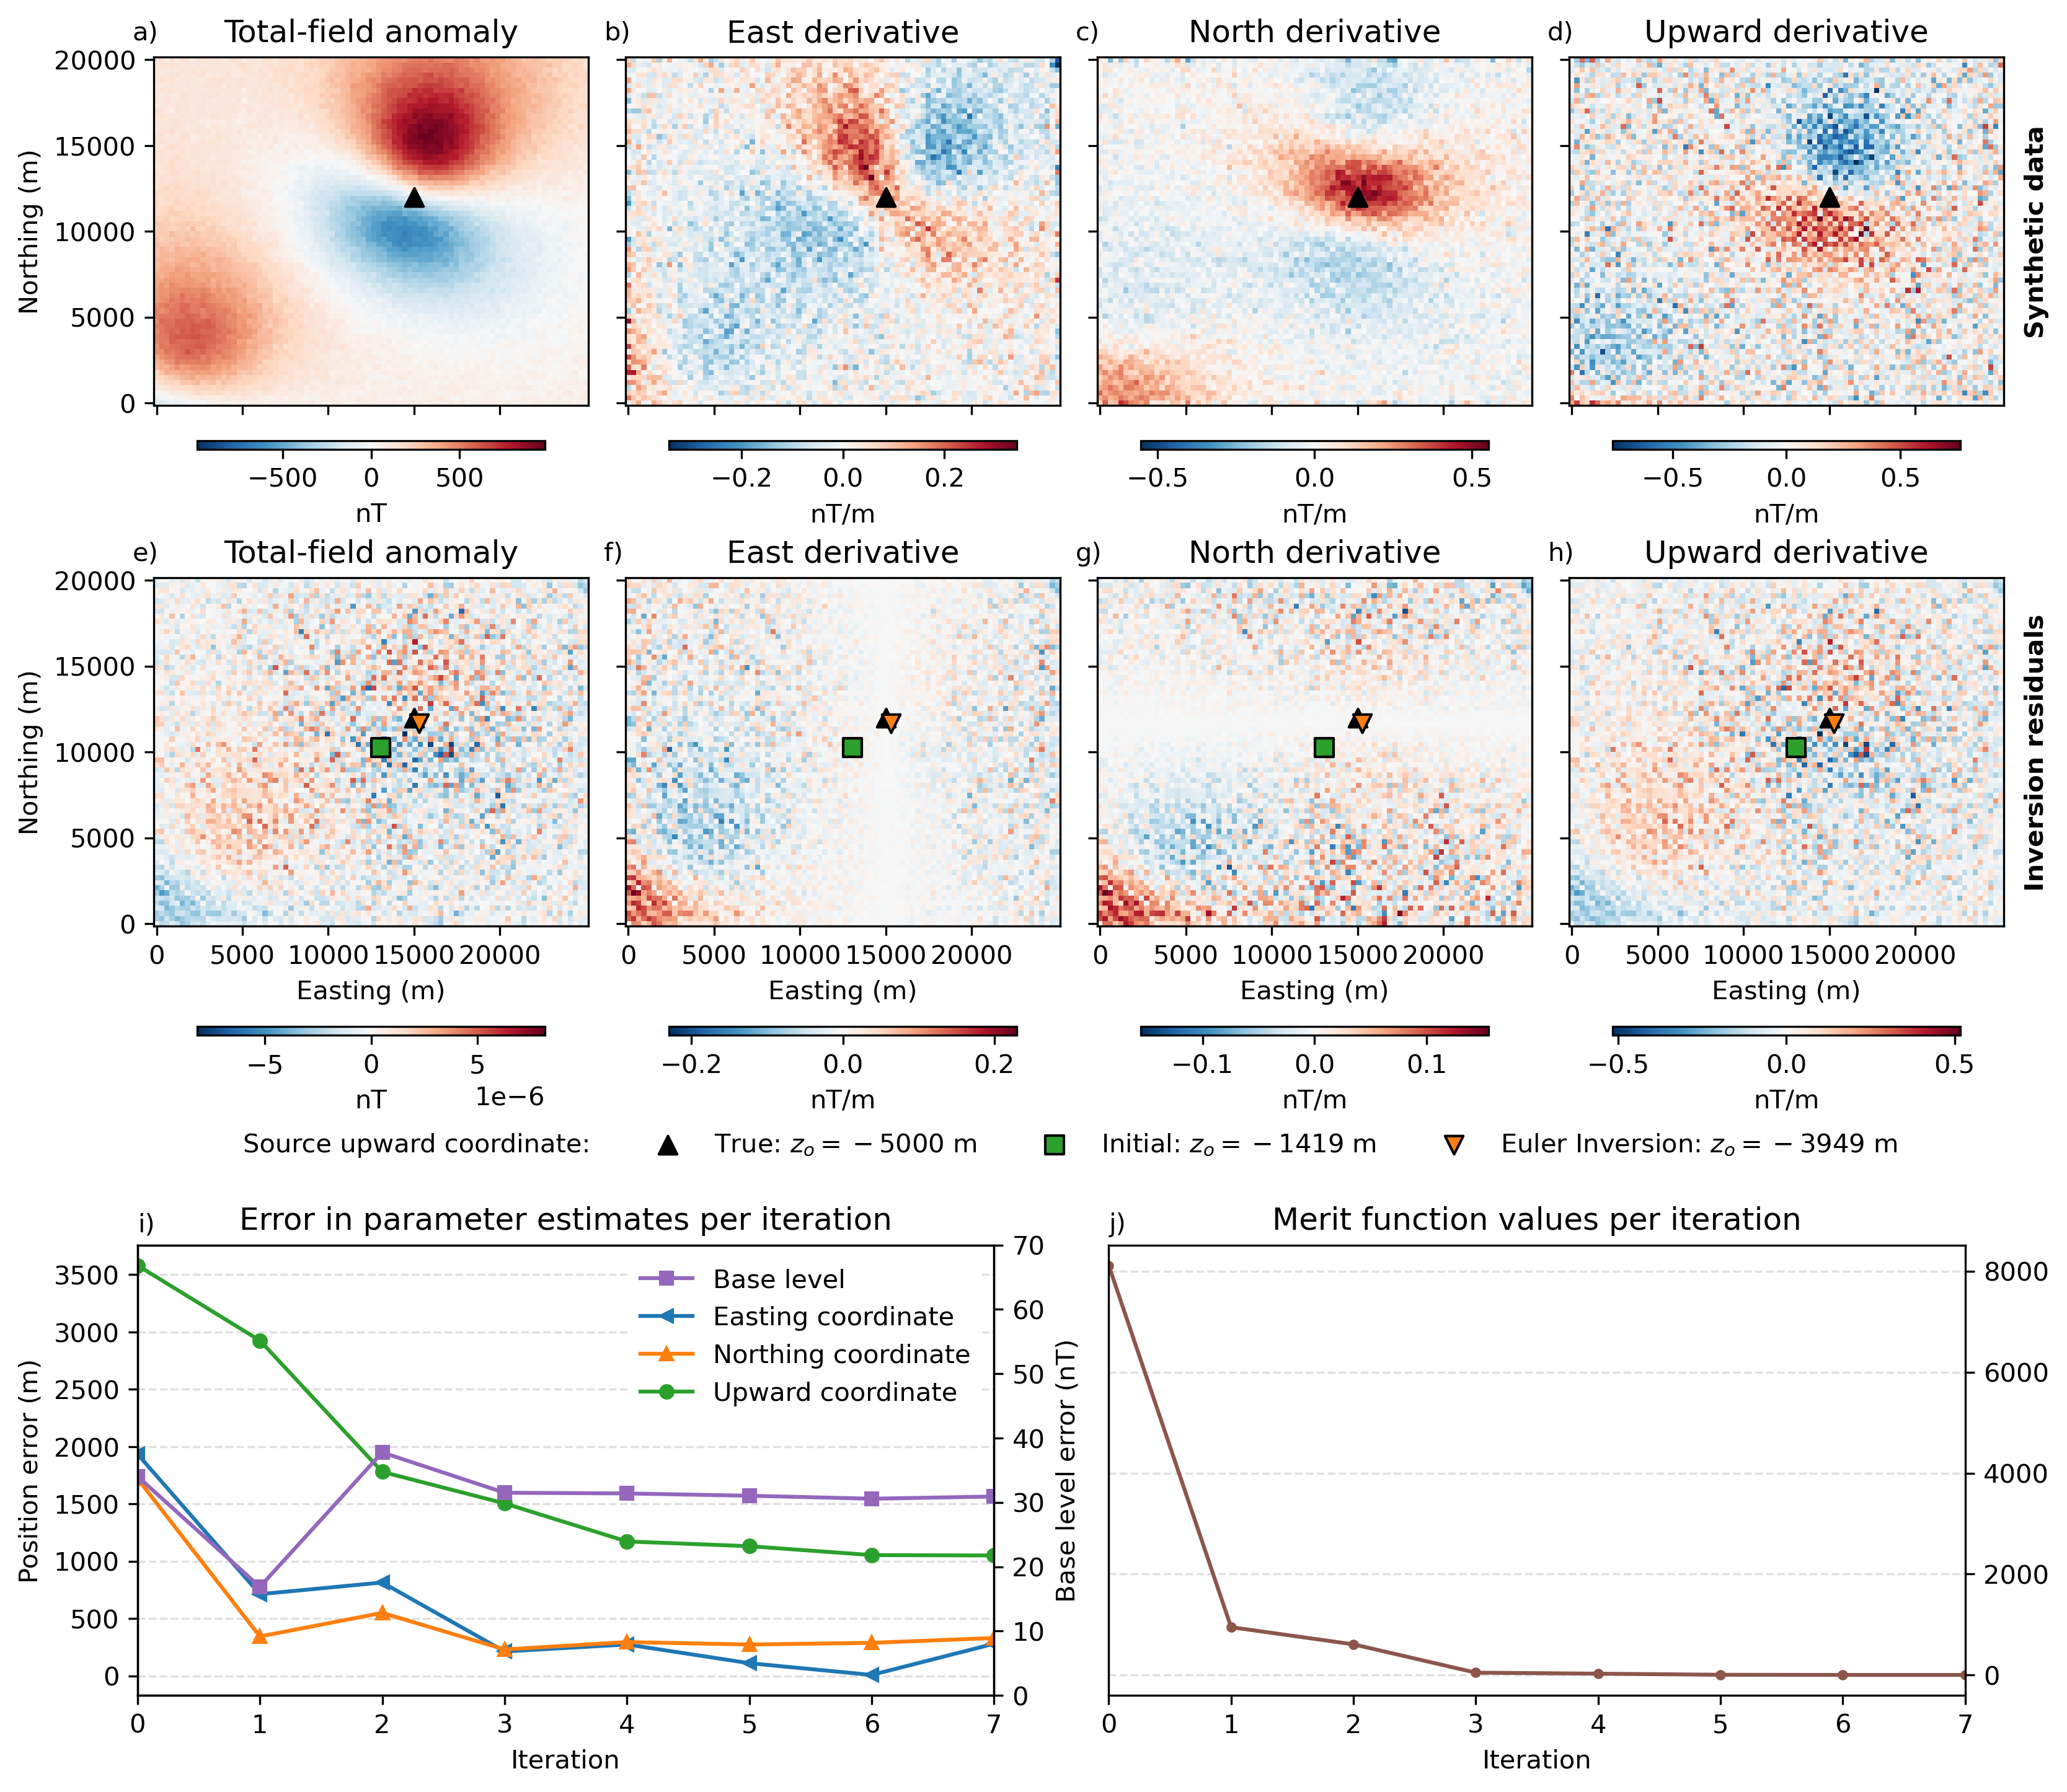
\includegraphics[width=1\linewidth]{figures/synthetic-proof-of-concept.png}
\caption{
    Data and results from the synthetic data test to demonstrate the performance of the method on a single target.
    a-d) The noise-corrupted synthetic total-field anomaly and its eastward, northward, and upward derivatives, respectively. The position of the dipolar source is marked by the black triangle.
    e-h) The Euler inversion residuals (observed data minus predicted data) for the total-field anomaly and its easting, northing, and upward derivatives, respectively. The black triangle shows the true location of the source, the green square shows the location estimated by Euler deconvolution, and the orange triangle shows the location estimated by Euler inversion.
    i) The error in the estimate of the easting (blue line), northing (orange line), and upward (green line) coordinates of the source and the base level (purple line) as a function of the Gauss-Newton iteration (Algorithm~\ref{alg:ei}).
    j) The value of the merit function $\Merit$ (Equation~\ref{eq:merit}) per Gauss-Newton iteration.
}
\label{fig:proof}
\end{figure}

The main goal of this synthetic data test is to demonstrate the general effectiveness of the Euler inversion method to estimate the position and base level of a single source.
To this end, we created a model composed of a single dipole located at
$(x_o = \SynProofTrueEast, y_o = \SynProofTrueNorth, z_o = \SynProofTrueUp)$
with a dipole moment magnitude of \SynProofInt{}, inclination of \SynProofInc{}, and declination of \SynProofDec{}.
The reference field direction was the same as the dipole moment direction.
The synthetic total-field magnetic anomaly data was calculated on a regular grid
with point spacing of \SynProofSpacing{} at a height of \SynProofHeight{}.
To the data, we added a base level of \SynProofTrueBase{} and
pseudo-random Gaussian noise with \qty{0}{\nano\tesla} mean and \SynProofNoise{} standard deviation.
The eastward and northward derivatives of the total-field anomaly grid were calculated with a central-difference scheme.
The upward derivative was calculated by Fast Fourier Transform (FFT).
The synthetic anomaly and its three derivatives are shown in Figures~\ref{fig:proof}a-d.

The Euler inversion method described in Algorithm~\ref{alg:ei} was applied to the synthetic data.
We chose a fixed structural index of $\eta=3$, which is the correct index for a magnetic dipole.
For data weights, we used \DefaultWeightsF{} for the total-field anomaly, \DefaultWeightsE{} for the east-derivative, \DefaultWeightsN{} for the north-derivative, and \DefaultWeightsU{} for the upward-derivative.
These weights were chosen to counteract the increased effect of noise on the derivatives, particularly the upward derivative which was calculated through FFT.
Figures~\ref{fig:proof}e-h show the inversion residuals after convergence was achieved ($L=\SynProofNIter{}$ iterations) for the total-field anomaly and its eastward, northward, and upward derivatives, respectively.
Also shown are the true source location, the initial source location (the Euler deconvolution result), and the predicted source location from Euler inversion.
The final Euler inversion prediction of the source location was $(x_o=\SynProofEstEast, y_o=\SynProofEstNorth, z_o=\SynProofEstUp)$ and the estimated base level was $b = \SynProofEstBase$, which is an improvement on the estimated values by Euler deconvolution (Figure~\ref{fig:proof}).

The convergence of the solution is shown in Figures~\ref{fig:proof}i-j.
The error in the estimated source coordinates and base level are shown in Figure~\ref{fig:proof}i.
The error in the $x_o$ (easting) and $y_o$ (northing) coordinates, as well as the base level, do not vary greatly from the initial solution.
However, the error in the $z_o$ (upward) coordinate drops from over \qty{1400}{\m} to less than \qty{400}{\m} in two iterations.
The merit function (Equation~\ref{eq:merit}) also drops sharply in value by two iterations, as can be seen in Figure~\ref{fig:proof}j, confirming the rapid convergence of the Euler inversion method.


\subsection{Effect of structural index choice}
\label{sec:si}

\begin{figure}[tb!]
\centering
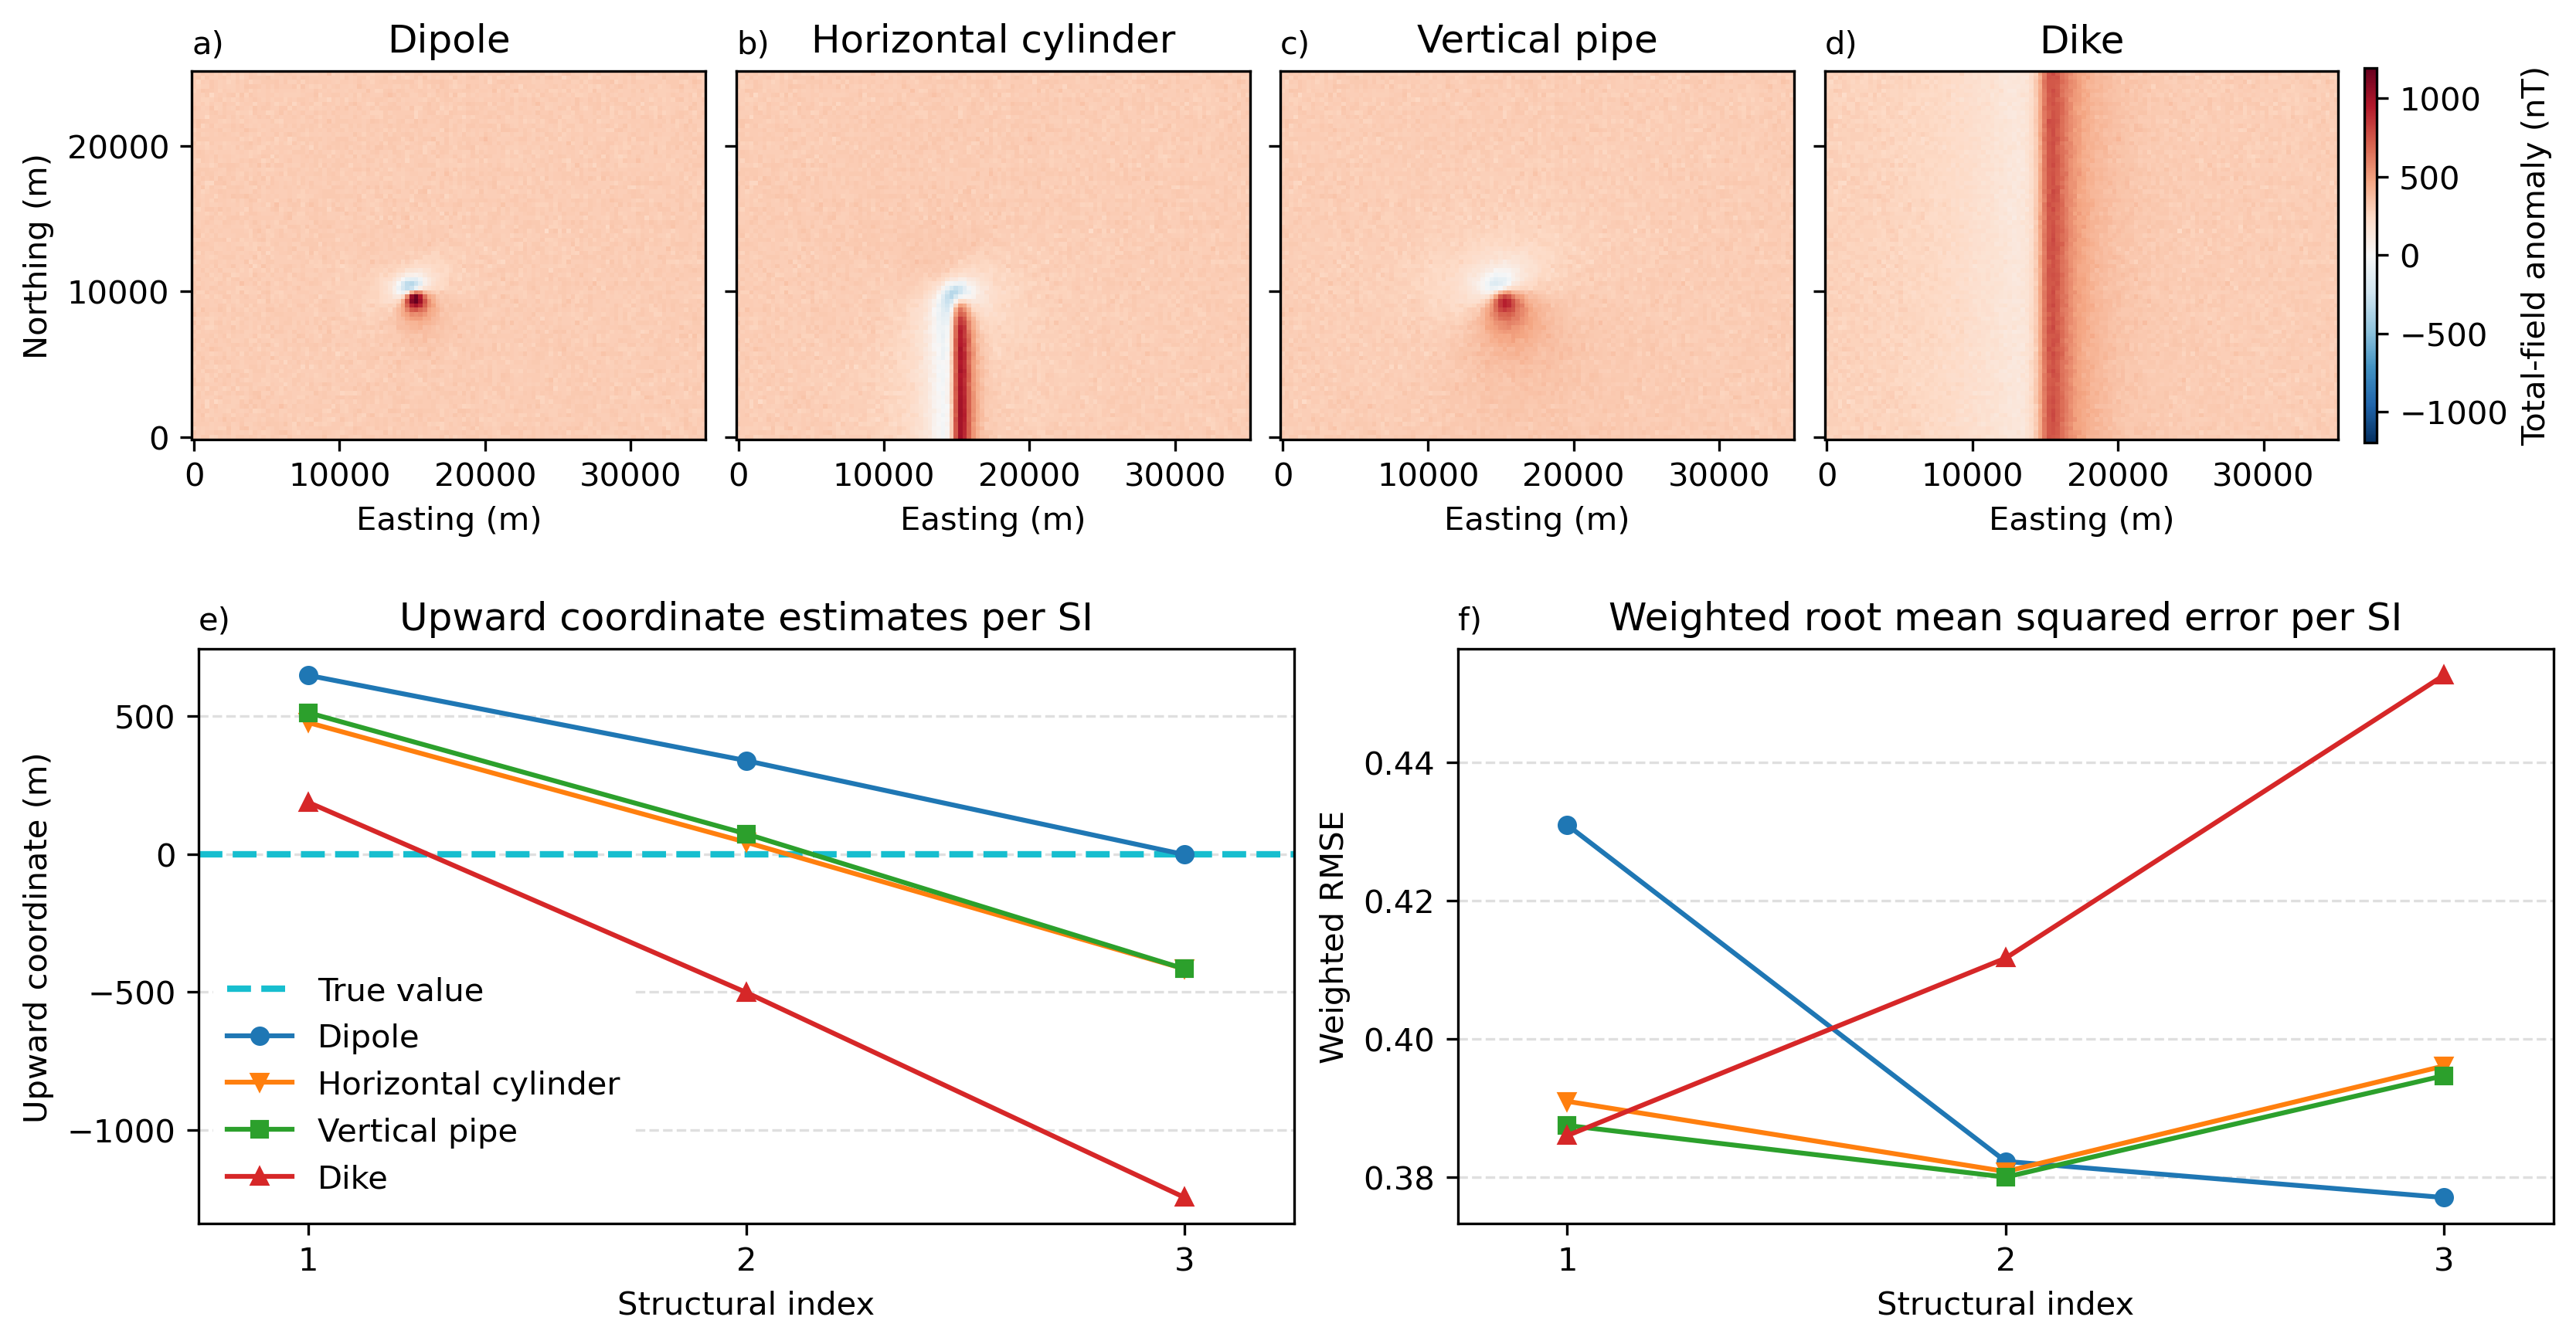
\includegraphics[width=1\linewidth]{figures/synthetic-structural-index.png}
\caption{
    Data and results from the synthetic data test using different values of structural index $\eta$ for different source types.
    a-d) Noise-corrupted total-field magnetic anomaly data caused by a dipole ($\eta=3$), a horizontal cylinder ($\eta=2$), a vertical pipe ($\eta=2$), and a vertical North-South dyke ($\eta=1$), respectively.
    e) Estimate of the upward source coordinate $z_o$ as a function of structural index for the dipole (blue line), horizontal cylinder (orange line), vertical pipe (green line), and dyke (red line).
    The true upward coordinate of the sources ($z_o = \SynSITrueUp$) is marked by the blue dashed line. Note that the $z_o$ estimate is closest to the true value when the correct structural index for each source type is used.
    f) The weighted root-mean-squared error (WRMSE; Equation~\ref{eq:wrmse}) as a function of structural index for the dipole (blue line), horizontal cylinder (orange line), vertical pipe (green line), and dyke (red line). The WRMSE is minimum for each source type when the correct structural index is used.
}
\label{fig:si}
\end{figure}

In this synthetic data test, we created datasets using four different models: a dipole, a horizontal cylinder composed of a right-rectangular prism stretched in the southward direction, a vertical pipe composed of a right-rectangular prism stretched in the downward direction, and a vertical dyke composed of a right-rectangular prism stretched in the southward, northward, and downward directions.
All models share the same true location of $(x_o=\SynSITrueEast, y_o=\SynSITrueNorth, z_o=\SynSITrueUp)$, base level of \SynSITrueBase, and induced magnetisation with inclination of \SynSIInc{} and declination of \SynSIDec.
The data were generated on a regular grid with spacing of \SynSISpacing, height of \SynSIHeight, and contaminated with pseudo-random Gaussian noise with \qty{0}{\nano\tesla} mean and \SynSINoise{} standard deviation. Figures~\ref{fig:si}a-d show the synthetic noise-corrupted total-field anomaly data.

We ran the Euler inversion method on each data grid three times, each time changing the structural index between one, two, and three.
Figure~\ref{fig:si}e shows the upward coordinate $z_o$ estimated for each of the four models as a function of the structural index $\eta$.
The Euler inversion estimated $z_o$ correlates with $\eta$, with larger values of the structural index leading to deeper source estimates.
Values closest to the true $z_o=\SynSITrueUp$ are achieved when the correct structural index is used ($\eta=1$ for the dyke, $\eta=2$ for the cylinder and pipe, and $\eta=3$ for the dipole).
Figure~\ref{fig:si}f shows the weighted root-mean-squared error (WRMSE; Equation~\ref{eq:wrmse}) at the final iteration of the Euler inversion method for all four models as a function of structural index.
The WRMSE is a measure of goodness-of-fit between the predicted total-field anomaly and its three derivatives and their observed counterparts.
The WRMSE is minimum for all four models when the correct structural index is used.


\subsection{Effect of random noise}
\label{sec:noise}

\begin{figure}[tb!]
\centering
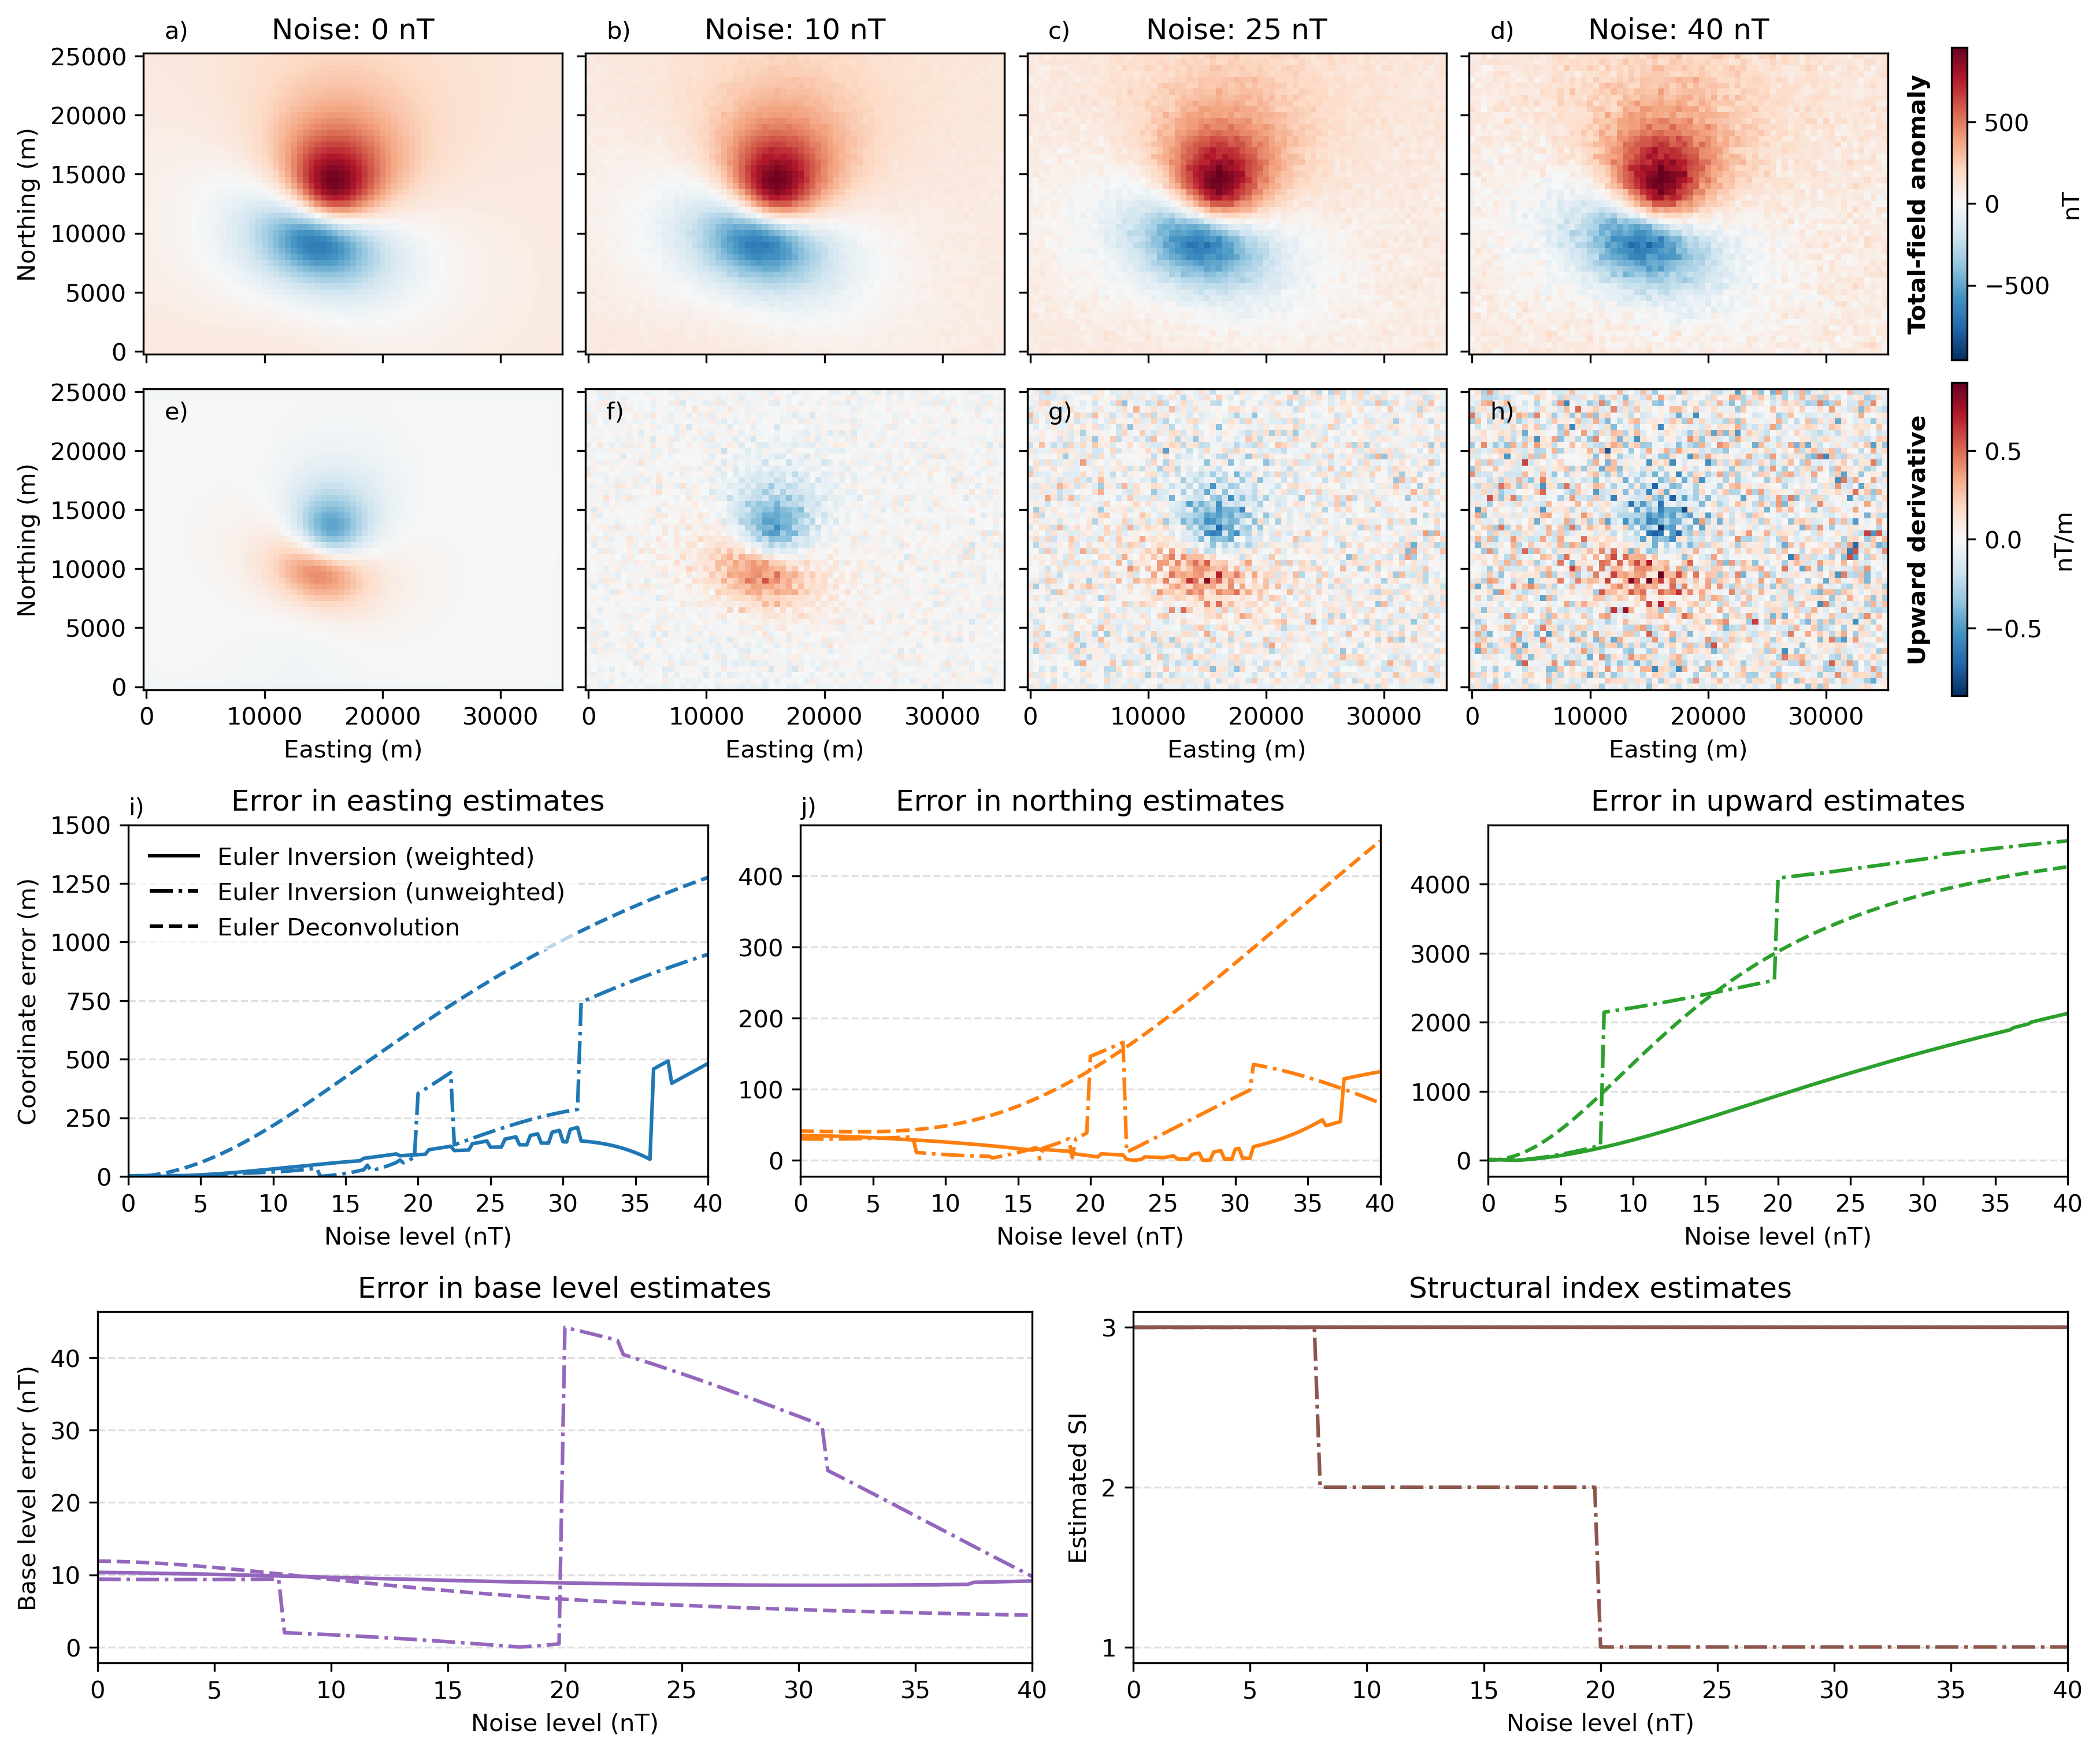
\includegraphics[width=1\linewidth]{figures/synthetic-noise-levels.png}
\caption{
    Data and results from the synthetic data test used to investigate the effect of high-frequency noise on the Euler inversion results.
    a-d) Noise-corrupted total-field magnetic anomaly of a dipolar source for noise levels \SynNoisePlotted.
    e-h) The upward derivative of the data in a-d, calculated by FFT.
    i-k) Error in the estimated easting, northing, and upward coordinates, respectively.
    l) Error in the estimated base level.
    m) The estimated structural index $\eta$ using Algorithm~\ref{alg:si}.
    The lines in i-m are the results for Euler deconvolution (dashed line), Euler inversion without data weights (dashed-dotted line), and Euler inversion with weights (solid line) \SynNoiseWeightsF{} for the total-field anomaly, \SynNoiseWeightsE{} for the eastward derivative, \SynNoiseWeightsN{} for the northward derivative, and \SynNoiseWeightsU{} for the upward derivative.
}
\label{fig:noise}
\end{figure}

We conducted another experiment to determine the effect of random high-frequency noise on the Euler inversion estimates.
To this end, we created synthetic data from a dipole model located at $(x_o=\SynNoiseTrueEast, y_o=\SynNoiseTrueNorth, z_o=\SynNoiseTrueUp)$ and with a dipole moment magnitude of \SynNoiseInt{}, inclination of \SynNoiseInc, and declination of \SynNoiseDec.
The total-field anomaly data were generated on a regular grid with a spacing of \SynNoiseSpacing{} and a constant height of \SynNoiseHeight.
The reference field direction was the same as the dipole moment direction.
A base level of \SynNoiseTrueBase{} was added to the data.
We generated different datasets by adding pseudo-random Gaussian noise with \qty{0}{\nano\tesla} mean and standard deviations varying from \SynNoiseMin{} to \SynNoiseMax{} with a step of \SynNoiseStep{}.
Figures~\ref{fig:noise}a-d show the synthetic data for noise levels \SynNoisePlotted, while Figures~\ref{fig:noise}e-h show the upward derivative calculated from the total-field anomaly through FFT.

On each dataset, we ran Euler deconvolution (Equation~\ref{eq:deconv-p}), Euler inversion with unit weights, and Euler inversion with weights \SynNoiseWeightsF{} for the total-field anomaly, \SynNoiseWeightsE{} for the eastward derivative, \SynNoiseWeightsN{} for the northward derivative, and \SynNoiseWeightsU{} for the upward derivative.
Both Euler inversion runs used the structural index estimation procedure (Algorithm~\ref{alg:si}).
Figures~\ref{fig:si}i-l show the error in the estimated easting, northing, and upward coordinates as well as the base level for each of the methods as a function of noise level.
The error in each of three coordinates raises sharply with noise level for Euler deconvolution, particularly for the upward $z_o$ coordinate.
The unweighted Euler inversion results vary less regularly but the present errors are just as large as Euler deconvolution for the upward coordinate.
However, the weighted Euler inversion presented overall smaller errors and a slower growth curve for the upward coordinate error than the other two methods.
The base level error is nearly constant at approximately \qty{10}{\nano\tesla} for Euler deconvolution and the weighted Euler inversion, but varies to as much as \qty{40}{\nano\tesla} for the unweighted Euler inversion.

Figure~\ref{fig:noise}m shows the estimated structural index $\eta$ for the weighted and unweighted Euler inversion as a function of noise level.
The unweighted Euler inversion estimated the wrong structural index $\eta=2$ from approximately noise level \qty{7}{\nano\tesla} and $\eta=1$ from approximately noise level \qty{20}{\nano\tesla}.
These jumps in the estimated structural index appear to correlate with jumps in the base level and $z_o$ coordinate errors.
The weighted Euler inversion was able to estimate the correct structural index ($\eta=3$) for all noise levels tested.


\subsection{Effect of interfering sources}
\label{sec:interf}

\begin{figure}[tb!]
\centering
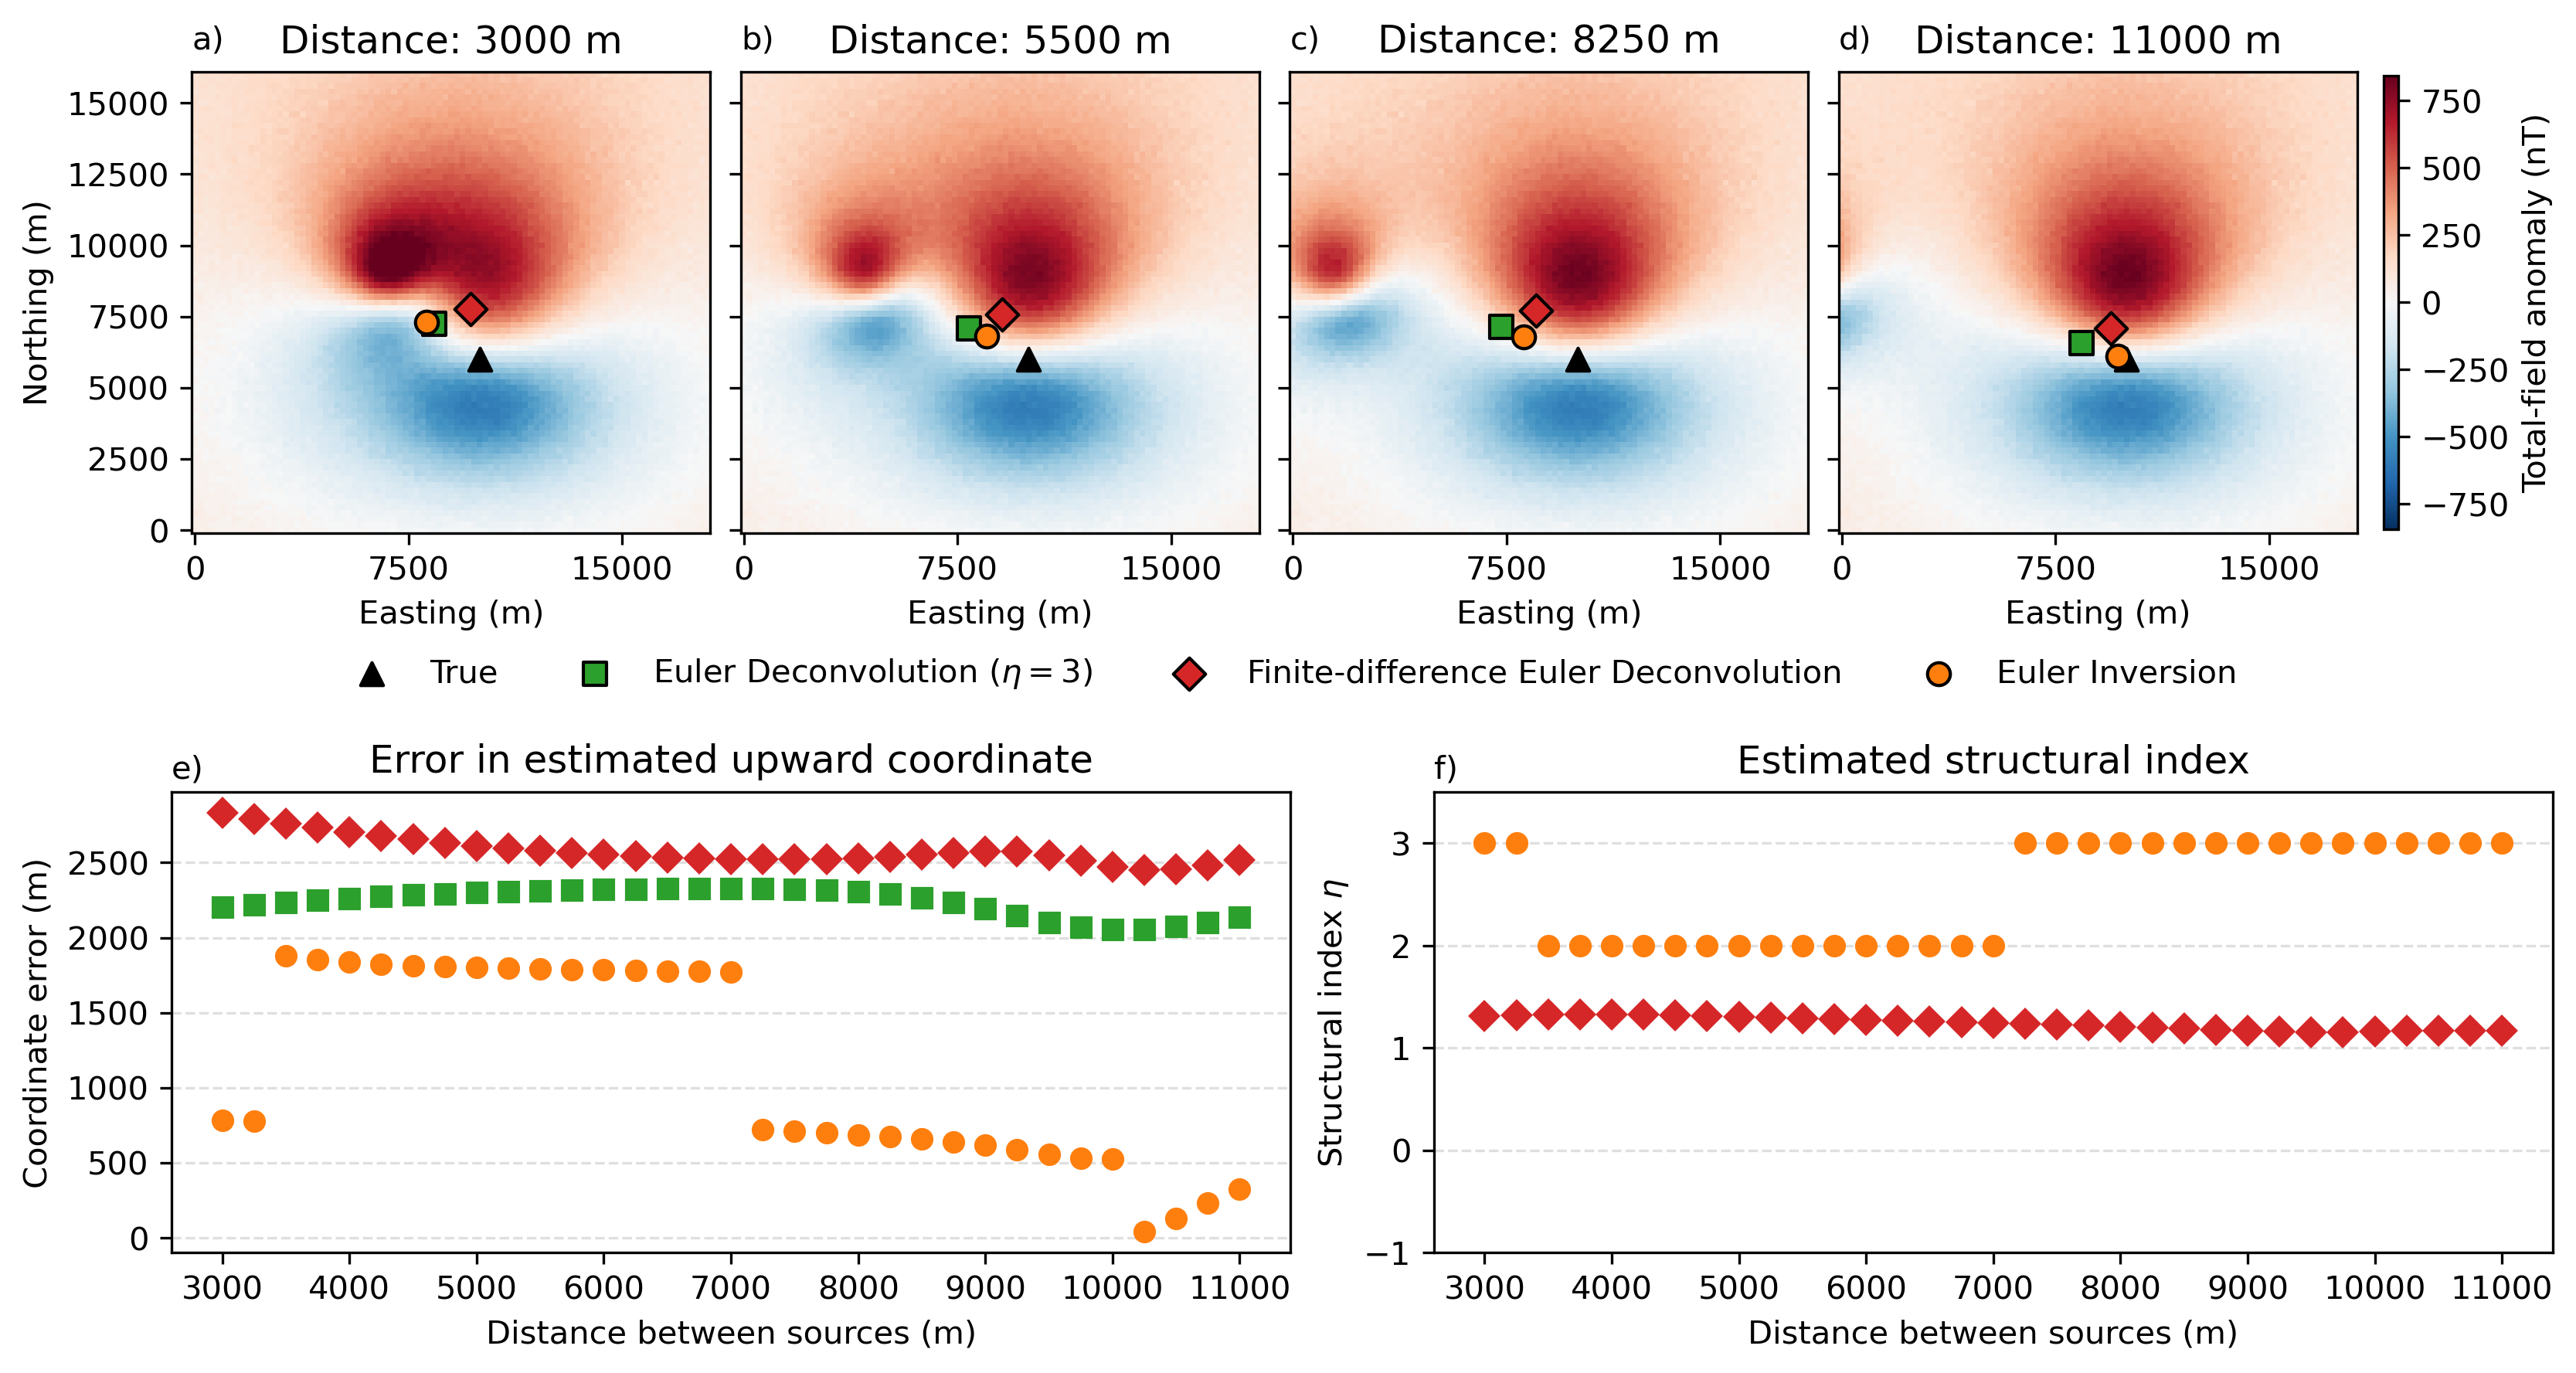
\includegraphics[width=1\linewidth]{figures/synthetic-interfering-sources.png}
\caption{
    Data and results from the synthetic data test used to investigate the effect of interfering sources inside the data window on the Euler inversion results.
    a-d) Noise-corrupted total-field magnetic anomaly for four models, each of which include the same central dipole but different interfering sources in the form of another dipolar source. Also plotted are the estimated positions from Euler deconvolution, finite-difference Euler deconvolution, and Euler inversion.
    e) The error in the estimated upward coordinate of the source $z_o$ for each of the Euler methods as a function of the model number.
    f) The estimated structural index $\eta$ for Euler inversion and finite-difference Euler deconvolution as a function of the model number.
    The true source location is represented by a black triangle, the Euler deconvolution result by a green square, the finite-difference Euler deconvolution result by a red diamond, and the Euler inversion result by an orange circle.
}
\label{fig:interf}
\end{figure}

Another common issue encountered during the application of Euler-based methods is the presence of interfering sources within the data window.
To test this effect on Euler inversion, we create four different synthetic total-field anomaly datasets.
All contain a main dipole located at $(x_o=\SynInterfTrueEast, y_o=\SynInterfTrueNorth, z_o=\SynInterfTrueUp)$ with a dipole moment amplitude of \SynInterfInt{}, inclination of \SynInterfInc, and declination of \SynInterfDec.
The reference field direction was the same as the dipole moment direction.
Each of the four models also contain a second dipolar source, simulating an interfering source in the data window, that is located at different places and depths relative to the main dipole.
The total-field anomaly data were generated on regular grids with a spacing of \SynInterfSpacing{} and at a constant height of \SynInterfHeight.
We added to all datasets a base level of \SynInterfTrueBase{} and pseudo-random Gaussian noise with \qty{0}{\nano\tesla} mean and \SynInterfNoise{} standard deviation.
Figures~\ref{fig:interf}a-d show the noise-corrupted total-field anomaly for each of the models.

On each dataset we, ran Euler deconvolution (Equation~\ref{eq:deconv-p} with structural index $\eta=3$), the finite-difference Euler deconvolution method of \citet{Gerovska2005}, and Euler inversion with the structural index estimation (Algorithm~\ref{alg:si}) and data weights of \DefaultWeightsF{} for the total-field anomaly, \DefaultWeightsE{} for the eastward derivative, \DefaultWeightsN{} for the northward derivative, and \DefaultWeightsU{} for the upward derivative.
The estimated easting and northing coordinates are shown in Figures~\ref{fig:interf}a-d.
For models 2 and 3, all three methods performed similarly in estimating the horizontal coordinates of the true source.
For models 1 and 4, the Euler deconvolution and finite-difference Euler deconvolution results are comparable, whilst the Euler inversion results are closer to the true source location.
Figure~\ref{fig:interf}e shows the error in the estimated upward coordinate for all three methods and four models.
The Euler inversion errors are consistently lower than those of both Euler deconvolution methods.
With the exception of model 2, the Euler inversion error on the upward coordinate are approximately half those of the Euler deconvolution methods.
Figure~\ref{fig:interf}f shows the estimated structural index for finite-difference Euler deconvolution and Euler inversion.
The finite-difference Euler deconvolution method consistently estimated values lower than $\eta=1$.
With the exception of model 2, Euler inversion was able to estimate the correct structural index ($\eta=3$) for all other models.


\subsection{Moving window procedure with multiple sources}
\label{sec:windows}

\begin{figure}[tb!]
\centering
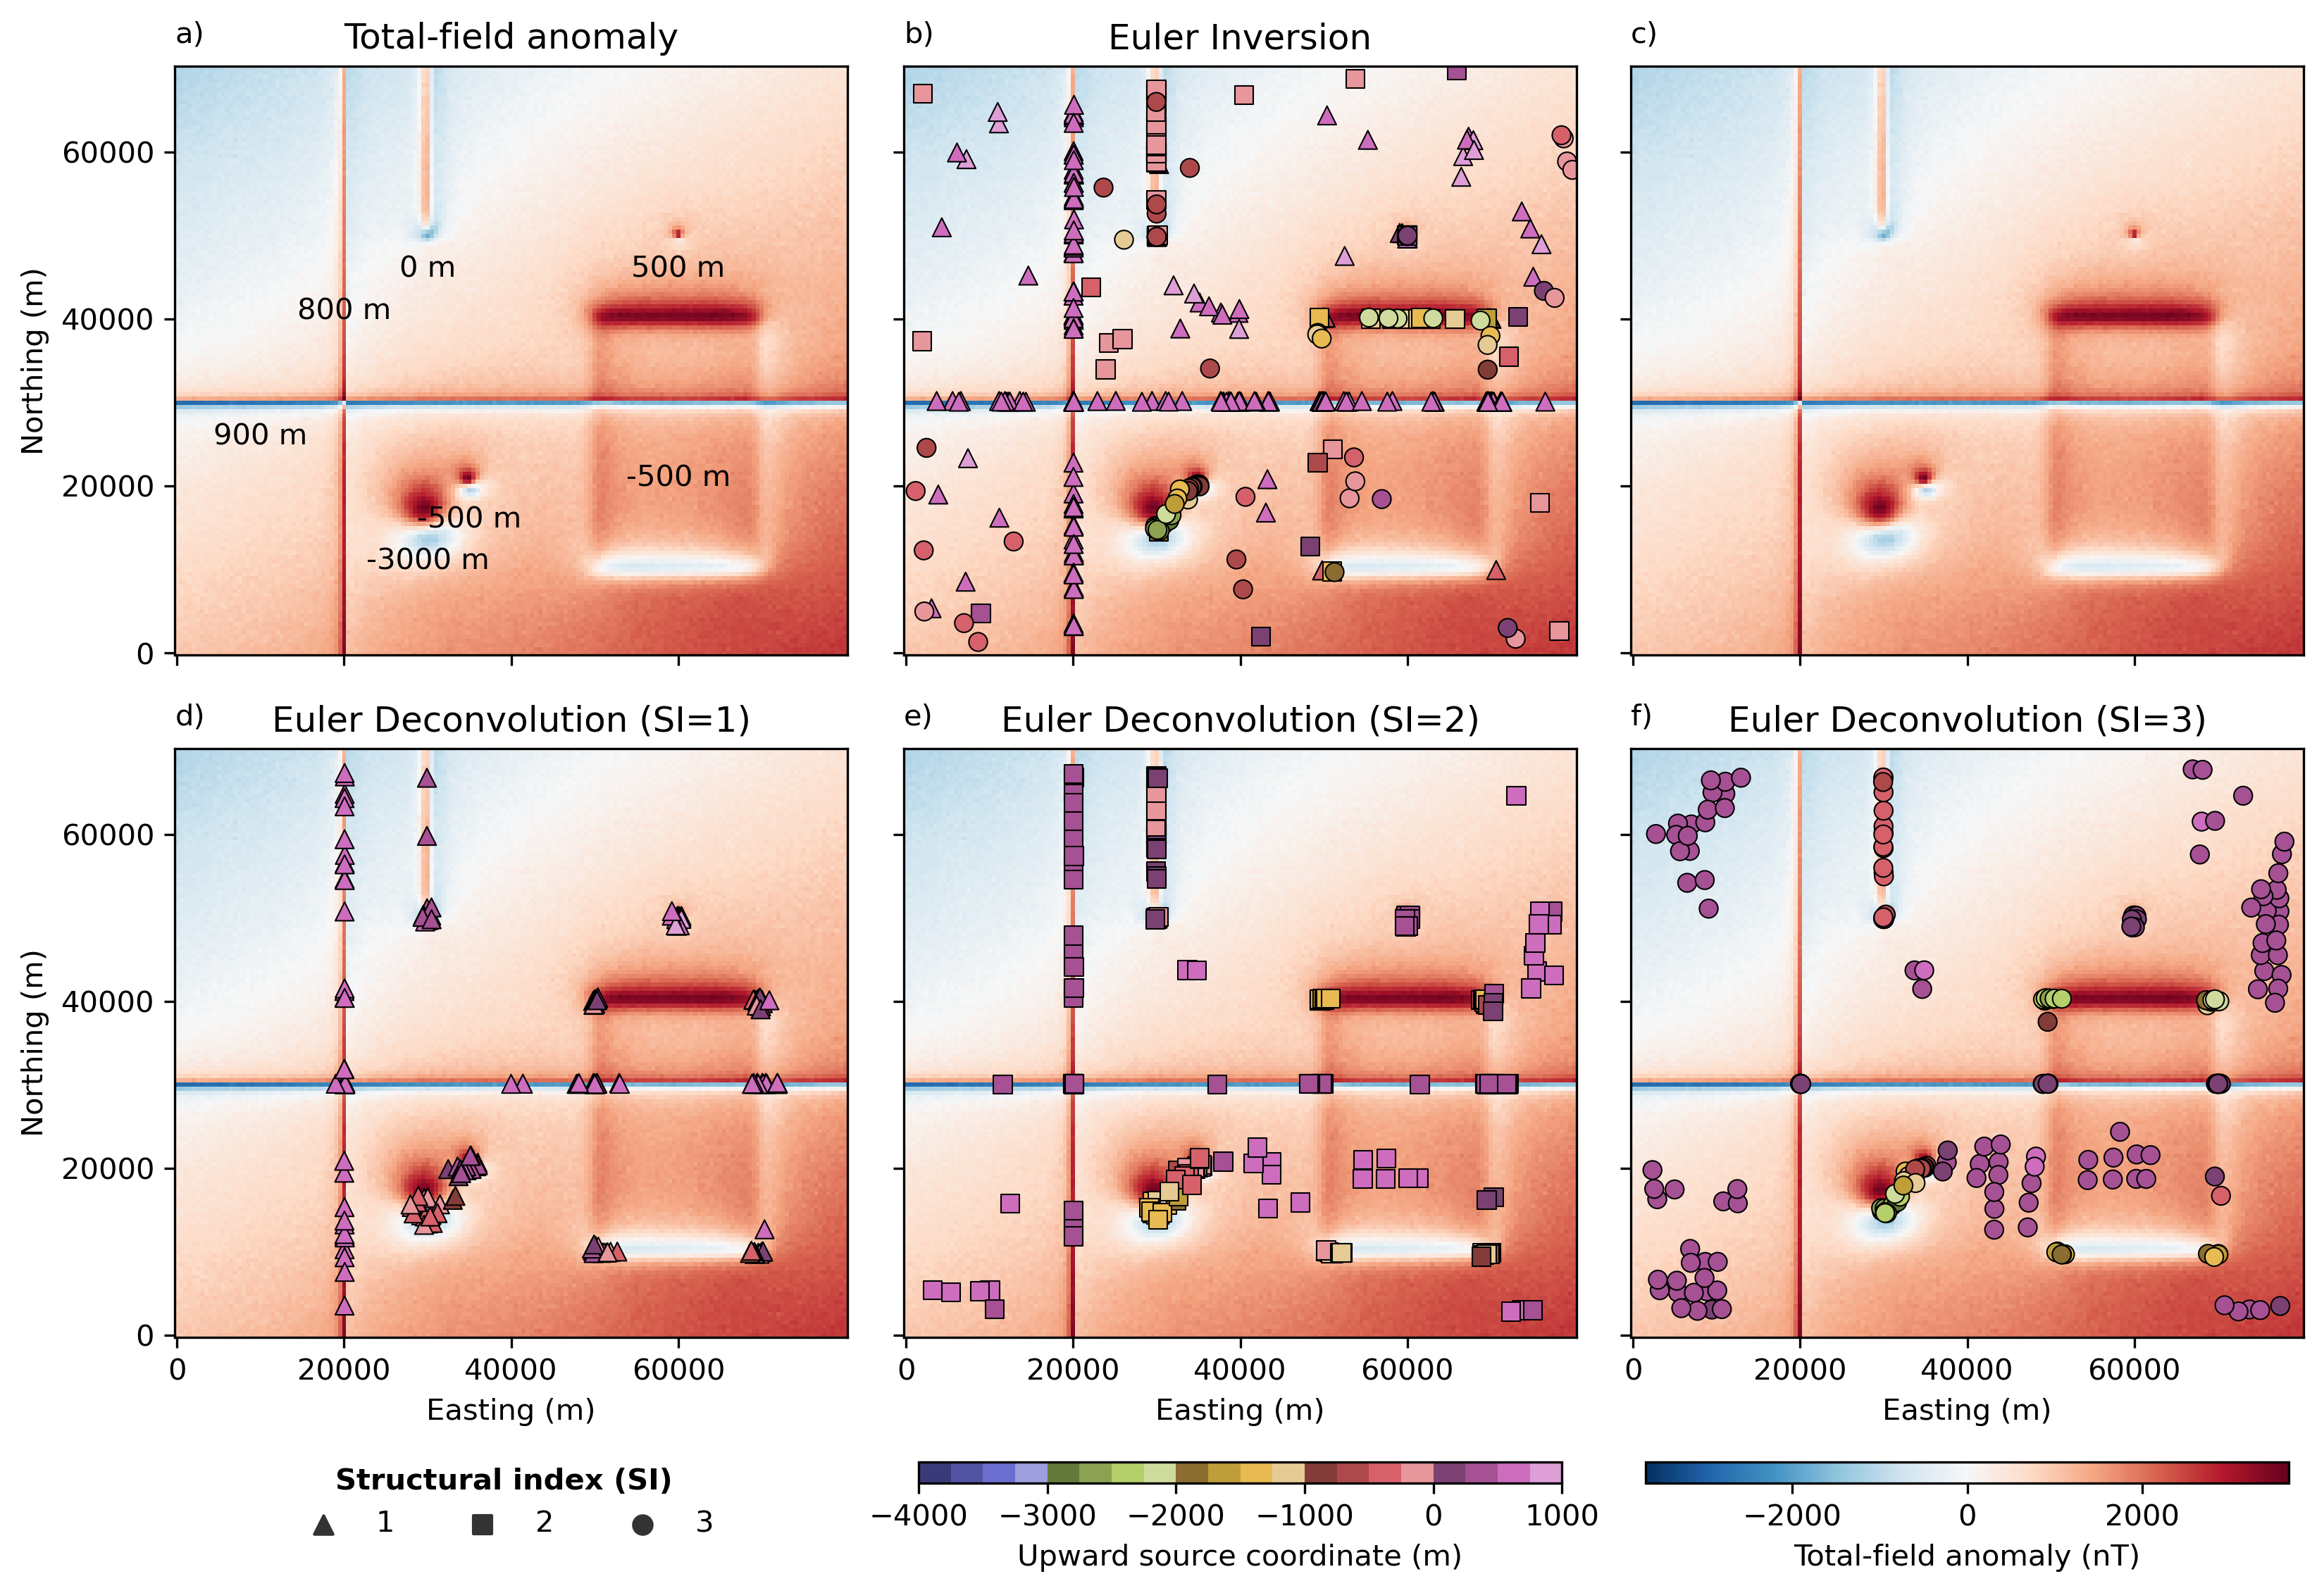
\includegraphics[width=1\linewidth]{figures/synthetic-windows.png}
\caption{
    Data and results from the synthetic data test using the moving window scheme (Algorithm~\ref{alg:window}).
    a) Noise-corrupted total-field magnetic anomaly generated from \SynWinNSources{} sources with overlapping signals, including dykes and dipoles. The true upward coordinate $z_o$ of each source is shown next to their respective anomalies.
    b-f) The estimated source locations from finite-difference Euler deconvolution, Euler inversion, Euler deconvolution ($\eta=1$), Euler deconvolution ($\eta=2$), and Euler deconvolution ($\eta=3$), respectively. The total-field anomaly is shown in the background for reference.
    The structural index of the solutions are represented by pentagons ($\eta=-1$),  diamonds ($\eta=0$),  triangles ($\eta=1$),  squares ($\eta=2$), and circles ($\eta=3$).
    For finite-difference Euler deconvolution (b), the structural index symbol is that of the closest integer to the estimated value.
    The color of each symbol represents the estimated upward coordinate $z_o$.
    The window size used was \SynWinWindowSize{} and the step between windows was \SynWinWindowStep{}.
}
\label{fig:windows}
\end{figure}

To simulate a more realistic dataset, we created a model composed of \SynWinNSources{} sources combining dipoles at various locations and depths and vertical dykes at various orientations.
All sources had induced magnetisation in the direction of the regional field with a inclination of \SynWinInc{} and declination of \SynWinDec{}.
The total-field anomaly of the model was calculated on a regular grid with a spacing of \SynWinSpacing{} and at a constant height of \SynWinHeight{}.
We added to the data a base level of \SynWinBase{}, pseudo-random Gaussian noise with \qty{0}{\nano\tesla} and \SynWinNoise{} standard deviation, and a regional field composed of a first-degree polynomial with angular coefficients of \SynWinRegionalE{} in the eastward and \SynWinRegionalN{} in the northward directions.
The noise-corrupted total-field anomaly data are shown in Figure~\ref{fig:windows}a.

To the dataset, we applied the moving window Euler inversion method (Algorithm~\ref{alg:window}), the finite-difference Euler deconvolution method of \citet{Gerovska2005}, and standard Euler deconvolution (using structural indices 1, 2, and 3).
Euler inversion was performed with data weights of \DefaultWeightsF{} for the total-field anomaly, \DefaultWeightsE{} for the eastward derivative, \DefaultWeightsN{} for the northward derivative, and \DefaultWeightsU{} for the upward derivative.
All three methods used the same moving window procedure described in Algorithm~\ref{alg:window} for the sake of comparison.
The windows had a size of \SynWinWindowSize{} and were moved by \SynWinWindowStep{} at a time.
The ratio of estimates kept to form the final solution was $\gamma=\SynWinKeepED$ for Euler deconvolution, $\gamma=\SynWinKeepFD$ for finite-difference Euler deconvolution, and $\gamma=\SynWinKeepEI$ for Euler inversion.

Figures~\ref{fig:windows}b-f show the estimated source positions and structural indices for finite-difference Euler deconvolution, Euler inversion, and Euler deconvolution with structural indices 1, 2, and 3, respectively.
The finite-difference method estimates a non-integer structural index, as a result Figure~\ref{fig:windows}b shows the closest integer value to the actual estimated $\eta$.
The finite-difference Euler deconvolution method underestimates the structural indices of all sources and, therefore, also underestimates their depths.
The finite-difference method solutions are also more scattered than their Euler deconvolution and Euler inversion counterparts.
The Euler deconvolution results are closer to the correct depths when the correct structural index is used.
They present larger dispersion than Euler inversion in areas where the signals of multiple sources overlap.
With the exception of the deeper dykes in the northwest and southeast and the small dipole with $z_o=\qty{-500}{\m}$, Euler inversion is able to estimate the correct structural index for most sources.
The upward coordinate estimates for Euler inversion are also closer than Euler deconvolution to their true values when the correct structural index was estimated.
Euler inversion notably estimates an incorrect $\eta$ and $z_o$ for smaller sources when there is a large amount of interference in the anomalies and for dykes that are deeper and produce a smoother signal.


\subsection{Aeromagnetic data from Rio de Janeiro}
\label{sec:rio}

\begin{figure}[tb!]
\centering
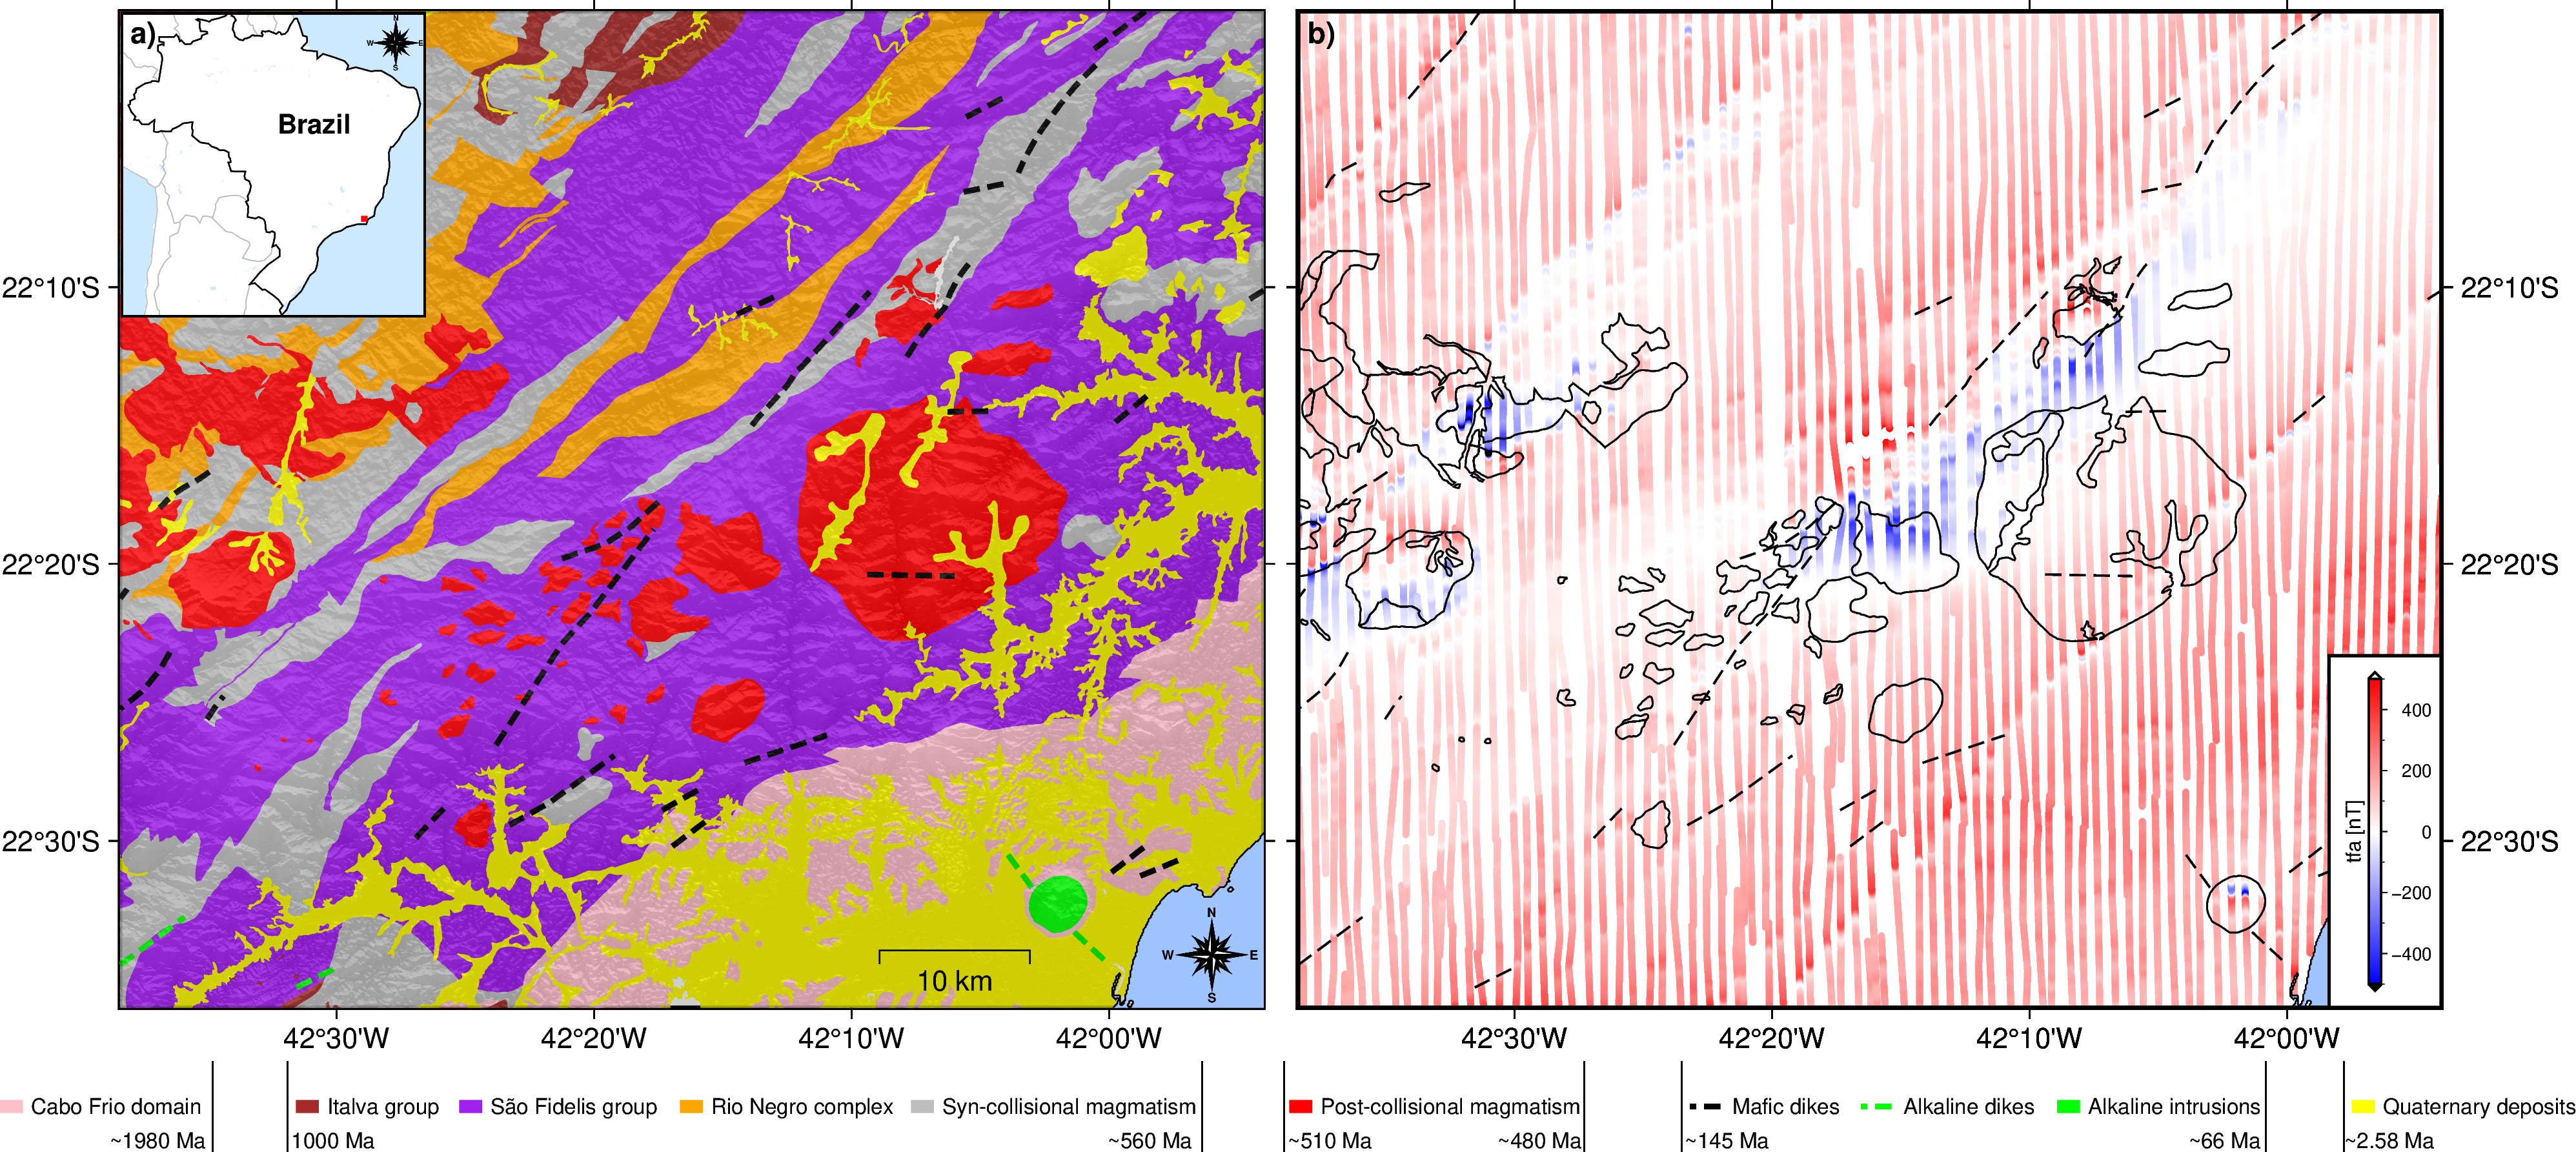
\includegraphics[width=1\linewidth]{figures/real-data-geology.png}
\caption{
  Geologic map and observed total-field magnetic anomaly data from the west of the state of Rio de Janeiro, Brazil.
  a) Simplified geologic map showing the main groups and dykes that outcrop in the region.
  In pink is the Cabo Frio domain, dark red is the Italva group, purple is the São Fidelis group, orange is the Rio Negro complex, gray is the syn-collisional magmatism, red is the post-collisional magmatism, green are alkaline intrusions, yellow are the Quaternary deposits, and the dashed lines are mafic and alkaline dykes.
  b) The aeromagnetic flight-line data, overlaid by the outlines of the post-collisional magmatism and alkaline intrusions (solid black lines) and dykes (dashed lines).
  The geologic map was modified from \citet{Heilbron2016} and \citet{Dantas2017}.
}
\label{fig:rio_context}
\end{figure}

\begin{figure}[tb!]
\centering
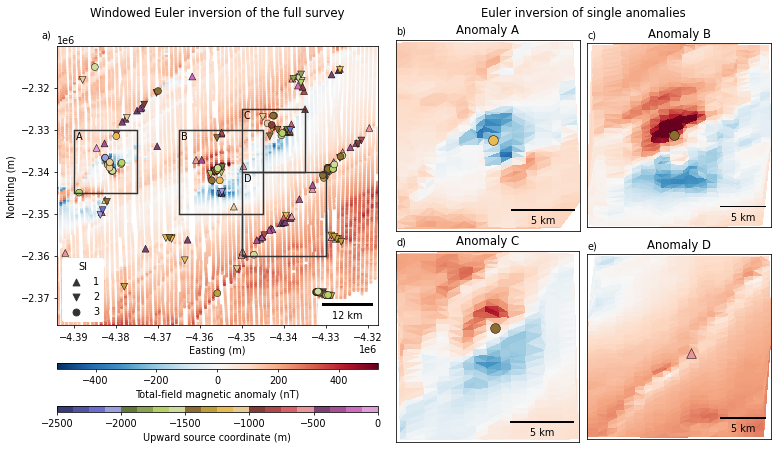
\includegraphics[width=1\linewidth]{figures/real-data-application.png}
\caption{
    Results of applying Euler inversion with a window size of \RioWindowSize{} and a window step of \RioWindowStep{} to the aeromagnetic data from Rio de Janeiro, Brazil.
    Estimated source locations and structural indices obtained from Euler inversion are shown as triangles ($\eta=1$), squares ($\eta=2$), and circles ($\eta=3$).
    The colour of each symbol represents the estimated depth below the surface of the Earth (topography).
    Also shown are the total-field anomaly flight-line data, the contours of the post-collisional magmatism and alkaline intrusions (solid black lines) and dykes (dashed lines).
    The purple squares highlight the A, B, C, and D anomalies that are discussed in the text.
}
\label{fig:rio_results}
\end{figure}

The geology of Rio de Janeiro state (Southeastern Brazil) consists primarily of
high-grade metamorphic rocks and granitoid magmatism related to the Ribeira
Belt (RB) \citep{Heilbron2020}.
Figure~\ref{fig:rio_context}a shows a simplified geologic map of the area, which was modified from \citet{Heilbron2016} and \citet{Dantas2017}.
The Ribeira Belt is traditionally interpreted as a thrust
belt formed by diachronous collisions mainly between the São Francisco and
Congo paleocontinents \citep{Heilbron2008, Trouw2000} or by an intracontinental
orogeny \citep[\textit{e.g.}][]{Meira2015, Meira2019}, during the Brasiliano
orogeny. This process culminated in an orogen-parallel, steep strike-slip shear
system \citep{EgydioSilva2005}, which deformed the Paleoproterozoic basement
rocks and reworked the Meso- to Neoproterozoic metasedimentary units (for example, the
Italva and São Fidelis groups) and syn-orogenic granitoid plutons (for example, the Rio
Negro complex) which formed during the orogeny \citep{Heilbron2003, Heilbron2020}.
These tectonic events imprinted a distinct NE-ENE-trending structural pattern
onto these rocks.

The late Neoproterozoic to Cambrian period witnessed post-orogenic magmatism
\citep[\textit{e.g.,}][]{Valeriano2011}, marking the final stages of the West
Gondwana amalgamation. After this, the region remained tectonically quiescent
until the Lower Cretaceous, when reactivation occurred with the emplacement of
the NE-trending Serra do Mar mafic dyke swarm, preceding the break-up of West
Gondwana and the opening of the South Atlantic Ocean \citep{Almeida2013}.
Lastly, thermal anomalies in the region during the Upper Cretaceous to
Paleocene period led to the emplacement of alkaline complexes and dykes
\citep{Thompson1998}.
The geological complexity of the Ribeira Belt, marked by the interplay of diverse tectonic
regimes and magmatic events (Figure~\ref{fig:rio_context}a), makes the Rio de Janeiro
region an ideal test case for Euler inversion.

We used aeromagnetic data from the state of Rio de Janeiro which are distributed by the Serviço Geológico do Brasil (\url{https://geosgb.sgb.gov.br}).
The data were collected in two phases: Subarea 1 was surveyed between March 25 and May 27, 1978, using
an Islander aircraft (PT-KRP), while Subarea 2 was surveyed between April 6 and
July 19, 1978, using a Bandeirante aircraft (PT-GKJ), both funded by the
Brazilian government.
As shown in Figure~\ref{fig:rio_context}b, the survey followed a pattern of north-south flight lines spaced approximately \qty{1}{\km} apart, with east-west tie lines.
Data were recorded at 100-meter intervals using a Geometrics G-803 magnetometer.
Some of the notable features of the data are the NE-SW linear features (interpreted here as dykes), which coincide with known dyke outcrops, and complex dipolar anomalies which coincide with some of the post-collisional magmatism and alkaline intrusions.
A subset of \RioNData{} data points were used in our analysis.

The data were not interpolated on a regular grid to avoid any smoothing effects that the interpolation might have on the linear features.
This could result in an over-estimation of their depth, as discussed in Section~\ref{sec:windows}.
Instead, we used the gradient-boosted equivalent sources method of \citet{Soler2021} to fit a model to the observed line data.
We then used the model to make predictions of the three spatial derivatives at the original measurement locations by a central-difference method with a coordinate shift of \RioDerivSpacing{}.
Further details about the data processing can be found in the source code archive that accompanies this article \url{https://doi.org/\ArchiveDOI} \citep{figshare}.

We performed the moving-window Euler inversion (Algorithm~\ref{alg:window}) on the observed total-field anomaly line data using windows of size of \RioWindowSize{} which were moved \RioWindowStep{} at a time.
The proportion of solutions kept was $\gamma=0.15$.
The inversion was performed with data weights of \RioWeightsF{} for the total-field anomaly, \RioWeightsE{} for the eastward derivative, \RioWeightsN{} for the northward derivative, and \RioWeightsU{} for the upward derivative.
To aid in the geological interpretation of the results, we converted the estimated upward source coordinates $z_o$ to depths below the surface of the Earth.
We did so by subtracting the estimated $z_o$ from the interpolated topographic height of the Shuttle Radar Topography Mission \citep[SRTM;][]{SRTM}.
The estimated positions and structural indices are shown in Figure~\ref{fig:rio_results}.

The estimated source positions shown in Figure~\ref{fig:rio_results} highlight the NE-SW lineaments as well as some of the more dipolar anomalies.
The lineaments are estimated with a mix of $\eta=1$, $\eta=2$, and $\eta=3$.
The southernmost lineament is mostly estimated with $\eta=1$ and depths suggesting that it does not outcrop in its southernmost parts (depths of \qtyrange{400}{600}{\m}), which is consistent with the geologic information in Figure~\ref{fig:rio_context}a.
The southernmost part of this lineament, in particular, has an estimated $\eta=3$, which is known to happen for deeper dykes in our synthetic data tests (Section~\ref{sec:windows}).
Conversely, the northernmost part of the lineament has a larger prevalence of $\eta=1$ with shallower depths which coincide with a known dyke outcrop.
Other known dyke outcrops coincide with estimated sources with $\eta=1$, however their depths range from \qtyrange{100}{300}{\m}.
This may be caused by an excess of smoothing in the vertical derivative or effects of noise in the estimated coordinates.
The lineaments in the northwestern part of the region are also highlighted by estimated sources.
However, their structural indices are a mix of $\eta=2$ and $\eta=3$, suggesting deeper sources.
This is inline with the geologic information, which includes no outcrops of linear structures in the area.

The dipolar anomalies are associated with post-collisional and alkaline intrusions, many of which are also cut by known outcropping dykes or have known dykes with magnetic signals that significantly overlap with the dipolar anomalies.
The Euler inversion estimated structural indices for them range from $\eta=2$ to $\eta=3$.
We have highlighted four dipolar anomalies, marked as A, B, C, and D in Figure~\ref{fig:rio_results}, to aid in our discussion.

\begin{itemize}
\item \textbf{Anomaly A:} Has a reversed polarity and linear feature to its north that is not associated with any known dyke outcrop.
The linear feature is highlighted by Euler inversion estimates with $\eta=1$ and depth of \qtyrange{300}{400}{\m}, which can be interpreted as a non-outcropping dyke.
The dipolar anomaly itself has Euler inversion solutions with $\eta=3$ and depth of \qtyrange{1000}{2000}{\m}.
The solutions in the centre of the anomaly present a shallower depth than the solutions to the north and south of the anomaly centre.
From the results on synthetic data in Section~\ref{sec:windows}, we can interpret the depth range to be caused by the moving window procedure and the effect of interfering sources.
The depth to the centre of the anomaly source is likely close to \qty{1000}{\m}.

\item \textbf{Anomaly B:} The dipolar anomaly is likely associated with a non-outcropping portion of the post-collisional magmatism.
The anomaly is cut by several NE-SW linear features, some of which overlap with known dyke outcrops.
The linear feature to the north is associated with Euler inversion results with $\eta=1$ and depths ranging from \qtyrange{300}{600}{\m}, suggesting a non-outcropping dyke.
At the centre of the anomaly are Euler inversion estimates with $\eta=3$ and depth estimate of approximately \qty{1400}{\m}.
The Euler inversion solutions surrounding these central solutions are likely caused by interference from other sources.

\item \textbf{Anomaly C:} A dipolar anomaly associated with an outcropping portion of the post-collisional magmatism.
There is a known outcropping dyke to the south of the anomaly, which is associated with Euler inversion estimates with $\eta=1$ and depths ranging from \qtyrange{500}{1000}{\m}.
These depth estimates are likely overestimated because of the interference of the dipolar anomaly.
The main anomaly has Euler inversion solutions with $\eta=2$ and $\eta=3$ and depths varying from
\qtyrange{1400}{1800}{\m}.
There is no clear indication of which of these estimates is more reliable.

\item \textbf{Anomaly D:} A small dipolar anomaly associated with an outcropping alkaline intrusion.
The Euler inversion estimates have $\eta=3$ and depths \qtyrange{1700}{2000}{\m}.
There are known outcropping dykes around the main intrusion but they have no discernible magnetic anomalies and no Euler inversion solutions associated with them.
\end{itemize}

Overall, the Euler inversion solutions in Figure~\ref{fig:rio_results} are consistent with the known geology in Figure~\ref{fig:rio_context}a.
The main linear features are mostly associated with Euler inversion estimates with $\eta=1$ and shallow depths, particularly where known dyke outcrops are located.
Deeper linear features are estimated with $\eta=2$ and $\eta=3$, which is consistent with the synthetic data results (Section~\ref{sec:windows}).
The dipolar anomalies have consistent Euler inversion estimates with $\eta=3$ when they are well isolated from interfering sources.
Otherwise, they are estimated with a mix of structural indices and depths, as was demonstrated in Section~\ref{sec:windows}.

%%%%%%%%%%%%%%%%%%%%%%%%%%%%%%%%%%%%%%%%%%%%%%%%%%%%%%%%%%%%%%%%%%%%%%%%%%%%%%%
\section{Conclusion}

Euler deconvolution is a widely used method for locating the sources of potential-field data, but under-performs in real-world scenarios due to its dependence on the chosen value of the structural index $\eta$ and its sensitivity to high-frequency noise and signal overlap.
We have developed a new method to solve Euler's homogeneity equation for the source position, base level, and integer structural index, which we call \textit{Euler inversion}.
Unlike Euler deconvolution, Euler inversion is also able to estimate the predicted field and its spatial derivatives, as well as assign different weights to each type of data.
The Euler inversion algorithm is computationally efficient because most of the large matrices involved in the computations are diagonal or block-diagonal.
We found that, in practice, the computation time of Euler inversion and Euler deconvolution are on the same order of magnitude.

Tests on synthetic data show that Euler inversion outperforms Euler deconvolution and finite-dif\-fer\-ence Euler deconvolution (a variant that estimates $\eta$ but does not rely on second-order derivatives) in terms of robustness to random noise and interfering sources inside the data window.
Our tests also show that the estimated $z_o$ coordinate is correlated with the structural index, as is the case for Euler deconvolution.
We have also found that the data misfit from Euler inversion is minimal when the integer structural index used is equal or close to the true one for idealized sources.
This led us to develop an algorithm for estimating the best integer structural index based on the data misfit.
A test on complex synthetic data from a model of dykes and dipoles with overlapping signals shows that Euler inversion is able to estimate the structural index and position of the sources within expected error bounds when the signal overlap is not larger than the data window.
For deeper dykes in particular, Euler inversion was not able to estimate the correct $\eta=1$, leading to an overestimation of the depths.

We applied Euler inversion to an aeromagnetic dataset from Rio de Janeiro, Brazil, to analyse its performance under real-world scenarios.
Euler inversion was able to locate the NE-SW linear features in the data with an $\eta=1$ which are associated with known dyke outcrops.
For the deeper linear features, Euler inversion was not able to estimate the correct $\eta=1$.
Some of the dipolar anomalies present in the data were picked out with $\eta=3$, while the sources with a large signal overlap with other features provided a mix of $\eta=2$ and $\eta=3$.
These results are consistent with the synthetic data tests and show the benefits and limitations of the proposed method.

Euler inversion outperforms other Euler-based methods in most cases.
However, it still suffers from some of the same limitations.
While Euler inversion is less sensitive to signal overlap, it still fails to correctly estimate the position and structural index when the overlap is large.
The windowing procedure still generates a large amount of spurious solutions which need to be filtered out.
This could be improved with techniques like the source detection method proposed by \citet{Castro2020}, for example.
Euler inversion can also be coupled with other inverse problems by following our methodology to add Euler's equation as a non-linear constraint.
This could help with issues of non-uniqueness and stability in traditional 3D inverse problems in potential-field methods.

%%%%%%%%%%%%%%%%%%%%%%%%%%%%%%%%%%%%%%%%%%%%%%%%%%%%%%%%%%%%%%%%%%%%%%%%%%%%%%%
\section*{Data availability statement}

The Python source code and data that were used to produce all results and
figures presented here are available at
\url{https://github.com/\GitHubRepository}
and \url{https://doi.org/\ArchiveDOI} \citep{figshare}
under the CC-BY license and the MIT license.
This study made use of the following open-source scientific software:
matplotlib \citep{matplotlib} and PyGMT \citep{pygmt} for generating figures and maps,
Numpy \citep{numpy} and Scipy \citep{scipy} for linear algebra,
Pandas for manipulating tabular data \citep{McKinney2010,pandas},
GeoPandas for reading and plotting shapefiles \citep{geopandas},
pyproj for data projection \citep{pyproj},
xarray \citep{xarray} for working with gridded data,
Verde \citep{verde} for moving windows and interpolation,
and Harmonica \citep{harmonica} for potential-field data processing and modeling.
The aeromagnetic and geologic data are available from Serviço Geológico do Brasil
(\url{https://geosgb.sgb.gov.br}) under a CC-BY-NC license.
The magnetic data are part of survey 1038 ``Projeto Aerogeofísico São Paulo -- Rio de Janeiro''.
Both are also available in our source code and data archive \citep{figshare}.


%%%%%%%%%%%%%%%%%%%%%%%%%%%%%%%%%%%%%%%%%%%%%%%%%%%%%%%%%%%%%%%%%%%%%%%%%%%%%%%
\section*{Acknowledgements}

% Thank the editors and reviewers after review.

We are indebted to the developers and maintainers of the open-source software
without which this work would not have been possible.
We thank Valéria C. F. Barbosa for many insightful discussions over the years which helped shape our research.
LU would like to thank Prof. Spiros Pagiatakis for being an incredible instructor and teaching him the mathematics which formed the foundations of this work during his undergraduate exchange at York University.
LU was supported in part by start-up grant PRPI 22.1.09345.01.2 from Universidade de São Paulo.
GFSJ was supported by scholarship 2021/08379-5 from the Fundação de Amparo à Pesquisa do Estado de São Paulo (FAPESP).
The opinions, hypotheses, and conclusions or recommendations expressed in this material are the responsibility of the authors and do not necessarily reflect the views of FAPESP.

\section*{CRediT author contributions}

\textbf{Leonardo Uieda:} Conceptualisation, Data curation, Formal analysis, Investigation, Methodology, Pro\-ject administration, Resources, Software, Supervision, Visualisation, Writing – original draft.

\noindent
\textbf{Gelson Ferreira Souza-Junior:} Data curation, Formal analysis, Resources, Software, Visualisation, Writing - original draft, Writing - review \& editing.

\noindent
\textbf{India Uppal:} Data curation, Formal analysis, Investigation, Software, Writing - review \& editing.

\noindent
\textbf{Vanderlei Coelho Oliveira Jr.:} Conceptualisation, Methodology, Writing - review \& editing.


\bibliographystyle{apalike-doi}
\bibliography{references}

\end{document}
